\chapter{TINJAUAN PUSTAKA}

\section{Tinjauan Pustaka}
Penelitian sebelumnya telah mengembangkan berbagai sistem pelacak kendaraan dengan berbagai macam pendekatan pada perangkat keras maupun perangkat lunak untuk berbagai aplikasi. Sebagai contoh, \cite{Ekhsan2022} merancang suatu sistem untuk melacak dompet dengan menggunakan TK-102 GPS \textit{Tracker}. Selain itu pelacak GPS juga dapat digunakan untuk aplikasi pada kapal kargo dan juga pada alat berat \cite{Zhang2013}\cite{Rani2021}. Pada penelitian ini, firmware GNSS \textit{tracker} yang dikembang difokuskan untuk melacak posisi bus kampus Trans Gadjah Mada.

Tim peneliti dari \textit{Vidyalankar Institute of Technology} telah merancang suatu sistem yang dapat mendeteksi lokasi dari kendaraan dan juga emisi \ce{CO} yang dihasilkan. Pada sistem yang dirancang, digunakan \textit{development board} Arduino Uno yang berbasis mikrokontroler ATmega328. Ketika kandungan gas \ce{CO} sudah melebihi ambang batas, sistem akan memutus pengiriman bahan bakar dan kemudian mengirimkan data koordinat dari modul GPS ke \textit{server} Apache yang telah dirancang \cite{Asha2022}.

Sebuah sistem \textit{speedometer} telah dirancang oleh \cite{Najmurrokhman2021}. Sistem tersebut menggunakan modul GPS untuk menghitung kecepatan dan koordinat lokasi kendaraan. Data kecepatan kendaraan didapat dari menghitung waktu yang dibutuhkan oleh kendaraan untuk berpindah dari satu titik ke titik lainnya. Jika dibandingkan dengan \textit{speedometer} pada aplikasi Google Maps, rata-rata dari selisih perhitungan kecepatan yang didapat adalah 3,9 km/jam. Selain itu, akurasi posisi yang didapat juga sudah cukup tinggi.

Penelitian yang dilakukan oleh \cite{Mukhtar2015} dari \textit{University of London} menggunakan mikrokontroler AT89S52 dari keluarga 8051. Digunakan modul GPS M-89 yang diatur untuk menerima isyarat transmisi satelit pada frekuensi 1575.42 MHz. Data yang diterima akan ditampilkan pada layar LCD dan dikirimkan dengan modul GSM. Kemudian, data yang telah diterima akan ditampilkan pada situs web.

Sistem yang dirancang pada penelitian \cite{Widya2016} menggunakan modul GPS u-Blox Neo 6m. Penelitian ini memiliki kesamaan, yaitu objek yang akan dilacak adalah kendaraan bus. Sama seperti penelitian-penelitian sebelumnya, pada penelitian ini hanya digunakan satu buah konstelasi GNSS, yaitu GPS.

Terakhir, penelitian \cite{Priono2017} membahas mengenai implementasi \textit{geofencing} untuk mengawasi pengiriman kendaraan pada perusahaan ekspedisi. Pada sistem yang dirancang, terdapat beberapa titik \textit{geofencing} di sepanjang rute perjalanan paket. Fitur serupa dapat diimplementasikan pada sistem pelacak Bus Trans Gadjah Mada. Sebagai contoh, sistem \textit{geofencing} untuk menentukan posisi halte saat ini.

Namun, pada penelitian-penelitian di atas hanya digunakan satu buah konstelasi GNSS, yaitu GPS. Oleh karena itu, pada penelitian ini akan dirancang sistem pelacak kendaraan berbasis GNSS \textit{multi-constellation} dengan menggunakan modul GNSS Teseo-LIV3FL dan mikrokontroler STM32 WL55JC. Selain itu, sistem \textit{geofencing} yang telah ada dapat dikembangkan lebih lanjut seperti dapat mendeteksi apakah kendaraan sedang berhenti di halte atau tidak.

\section{Dasar Teori}
\subsection{\textit{Firmware}}
\textit{Firmware} adalah suatu jenis perangkat lunak yang memberikan akses untuk kendali level rendah pada suatu komputer khusus, baik itu untuk menangani perangkat lunak lain atau untuk tujuan komputasi yang lebih spesifik. Perangkat lunak ini dapat ditemukan pada berbagai perangkat keras seperti komputer, sistem tertanam, periferal, dan sejenisnya. Sebagai catatan, \textit{firmware} berada di dalam memori \textit{non-volatile}.

ROM BIOS adalah salah satu contoh \textit{firmware} yang berfungsi untuk melakukan inisialisasi perangkat keras ketika komputer dihidupkan, dan memungkinkan pengguna untuk menambahkan program-program lain dengan level yang lebih tinggi di masa depan. Di sisi lain, \textit{firmware} pada sistem tertanam adalah satu-satunya perangkat lunak yang berjalan pada sistem tersebut.

Namun, penting untuk diingat bahwa \textit{firmware} dan sistem operasi sebenarnya merupakan dua hal yang berbeda, meskipun seringkali dianggap sebagai satu hal yang sama oleh beberapa orang. Sistem operasi merupakan perangkat lunak yang berjalan di atas \textit{firmware}, sedangkan \textit{firmware} sendiri bertanggung jawab untuk kendali fungsi dasar pada perangkat keras \cite{Davidson1978}.

\subsubsection{Bahasa Pemrograman C}
Bahasa C (dibaca "si") adalah bahasa pemrograman \textit{general-purpose} tingkat tinggi yang dikembangkan oleh Dennis Ritchie pada tahun 1972. Hingga saat ini, bahasa C adalah salah satu bahasa pemrograman yang paling banyak digunakan \cite{SO2022} untuk berbagai macam pengembangan seperti pengembangan \textit{firmware} pada sistem tertanam. Bahasa C sangat populer karena memiliki fleksibilitas, kekompakan, dan efisiensi yang sangat tinggi.

Pada awalnya, Bahasa C hanya dirancang untuk implementasi pada sistem operasi \cite{Ritchie1993}. Namun, dengan mekanisme \textit{data abstraction}, memungkinkan pengembangan aplikasi pada level tinggi maupun rendah. Sebagai contoh, anggota \textit{struct} dapat ditata sedemikian rupa agar sesuai dengan alamat \textit{port} dari perangkat keras. Selain itu, bahasa C juga menawarkan operasi tingkat rendah seperti \textit{bit shift}, logika AND, dan lainnya.

Bahasa C sering digunakan dalam pengembangan \textit{firmware} pada mikrokontroler karena memungkinkan pengembang untuk melakukan pemrograman pada tingkat register dan memori. Kendali langsung terhadap perangkat keras memungkinkan pengembang untuk merancang program dengan performa tinggi dan efisien. Bahasa C juga dapat diandalkan dalam mengakses perangkat keras yang terdapat dalam sistem tertanam. Selain itu, bahasa C juga populer untuk pengembangan aplikasi tingkat rendah seperti sistem operasi, perangkat lunak sistem, dan program pengontrol perangkat keras lainnya.

Saat ini, bahasa C terus digunakan dan dianggap sebagai bahasa pemrograman yang esensial bagi pengembang perangkat lunak. Bahasa C sangat fleksibel, ringkas, dan efisien sehingga dapat digunakan dalam berbagai proyek perangkat lunak yang kompleks \cite{Deitel2016}. Kepopuleran bahasa C juga didukung oleh adanya \textit{compiler} yang tersedia untuk berbagai \textit{platform} sistem operasi, sehingga bahasa ini dapat digunakan pada berbagai sistem operasi seperti Windows, Linux, macOS, dan sebagainya.

\subsection{Teknologi GNSS}
\textit{Global Navigation Satellite System} (GNSS) adalah teknologi yang sangat penting dan telah digunakan secara luas dalam berbagai aplikasi. Sistem ini digunakan untuk menentukan posisi di permukaan bumi dengan menggunakan konstelasi satelit sebagai referensi. Contoh GNSS yang paling terkenal adalah \textit{Global Positioning System} (GPS) milik Amerika Serikat, namun terdapat lima sistem GNSS lainnya yang dikembangkan oleh negara-negara lain, yaitu Galileo (Uni Eropa), BeiDou (Republik Rakyat Tiongkok), GLONASS (Federasi Rusia), IRNSS (India), dan QZSS (Jepang) \cite{NationalCoordinationOfficeforSpace-BasedPositioning2021}.

Sistem GNSS bekerja dengan cara mengobservasi jarak antara penerima dengan satelit menggunakan isyarat radio pada pita frekuensi L \cite{TheEuropeanGlobalNavigationSatelliteSystemsAgency2021}. Satelit GNSS akan terus memancarkan isyarat radio pada pita frekuensi L yang dapat diterima oleh penerima GNSS. Isyarat tersebut kemudian dihitung waktu tempuhnya oleh penerima GNSS untuk menentukan jarak antara penerima dan satelit. 

\begin{figure}[H]
	\centering
	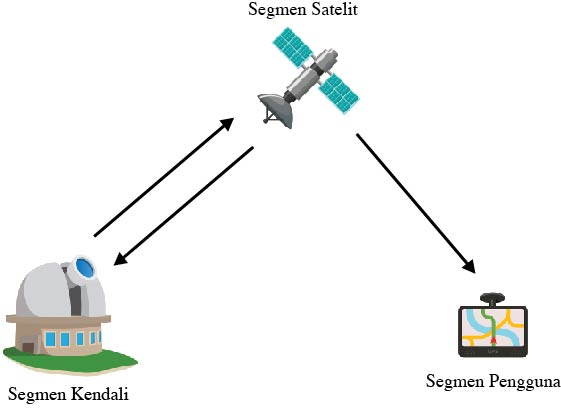
\includegraphics[width=8cm]{contents/chapter-2/gnss_segment.jpg}
	\caption{Segmen GNSS}
	\label{Fig: gnss_segment}
\end{figure}

Sistem GNSS memiliki tiga segmen yang saling terkait, yaitu segmen satelit, segmen kendali, dan segmen pengguna. Segmen satelit bertanggung jawab sebagai pemancar sinyal, yang diterima oleh segmen pengguna untuk menentukan posisi dan waktu. Sedangkan, segmen kendali mengawasi dan mengontrol kinerja satelit dengan memastikan akurasi sinyal yang diterima oleh pengguna. Ketiga segmen ini saling berkaitan dan dibutuhkan untuk memastikan keakuratan dan keandalan sistem GNSS. Gambar \ref{Fig: gnss_segment} memperlihatkan hubungan antara ketiga segmen GNSS tersebut.

\subsubsection{Orbit GNSS}
Ketinggian orbit dari setiap konstelasi GNSS adalah parameter untuk membagi orbit GNSS menjadi tiga kategori utama. Karakteristik tersebut memengaruhi penundaan waktu antara isyarat yang dipancarkan dan diterima yang ditunjukan oleh Gambar \ref{Fig: alt-comp}. Waktu penundaan didapat dari persamaan $t_d = \frac{2d}{c}$ dengan $d$ adalah ketinggian orbit satelit dan $c$ adalah kecepatan cahaya. Pengelompokan jenis orbit untuk setiap konstelasi GNSS ditunjukan oleh Tabel \ref{Tab: gnss-orbit}.

\begin{table}[H]
	\caption{Orbit dan Ketinggian setiap Konstelasi \cite{Li2019} \cite{Bury2019}}
	\vspace{0.5em}
	\centering
	\begin{tabular}{ccccc}
		\hline
		\textbf{GNSS} &\textbf{Tipe Orbit} & \textbf{Ketinggian (km)} & \textbf{Satelit} & \textbf{Total Satelit}\\
		\hline 
		\textbf{GPS} & MEO & 20.180 & 24 & 24\\
		\textbf{GLONASS} & MEO & 19.100 & 24 & 24\\
		\textbf{GALILEO} & MEO & 23.220 & 30 & 30\\
		\textbf{Beidou} & GEO & 35.786 & 3\\
		& IGSO & 35.786 & 3 & 30\\
		& MEO& 21.528 & 24\\
		\textbf{QZSS} & IGSO &32.000 s.d. 40.000 & 5 & 5\\
		\hline
	\end{tabular}
	\label{Tab: gnss-orbit}
\end{table}

\textbf{\textit{Low Earth Orbit} (LEO)} adalah satelit yang mengorbit Planet Bumi dengan ketinggian 500 sampai dengan 2000 km. Keuntungan yang dimiliki oleh satelit dengan orbit LEO adalah waktu penundaan antara isyarat dipancarkan dengan diterima sebentar, dapat beroperasi dengan daya rendah, dan biaya pemeliharaan yang murah. Kekurangan dari satelit dengan orbit LEO adalah dibutuhkan lebih banyak satelit untuk mencakup daerah operasi yang lebih luas. Sistem LEO dapat dikelompokan lebih lanjut berdasarkan frekuensi isyaratnya, yaitu:

\begin{figure}[H]
	\centering
	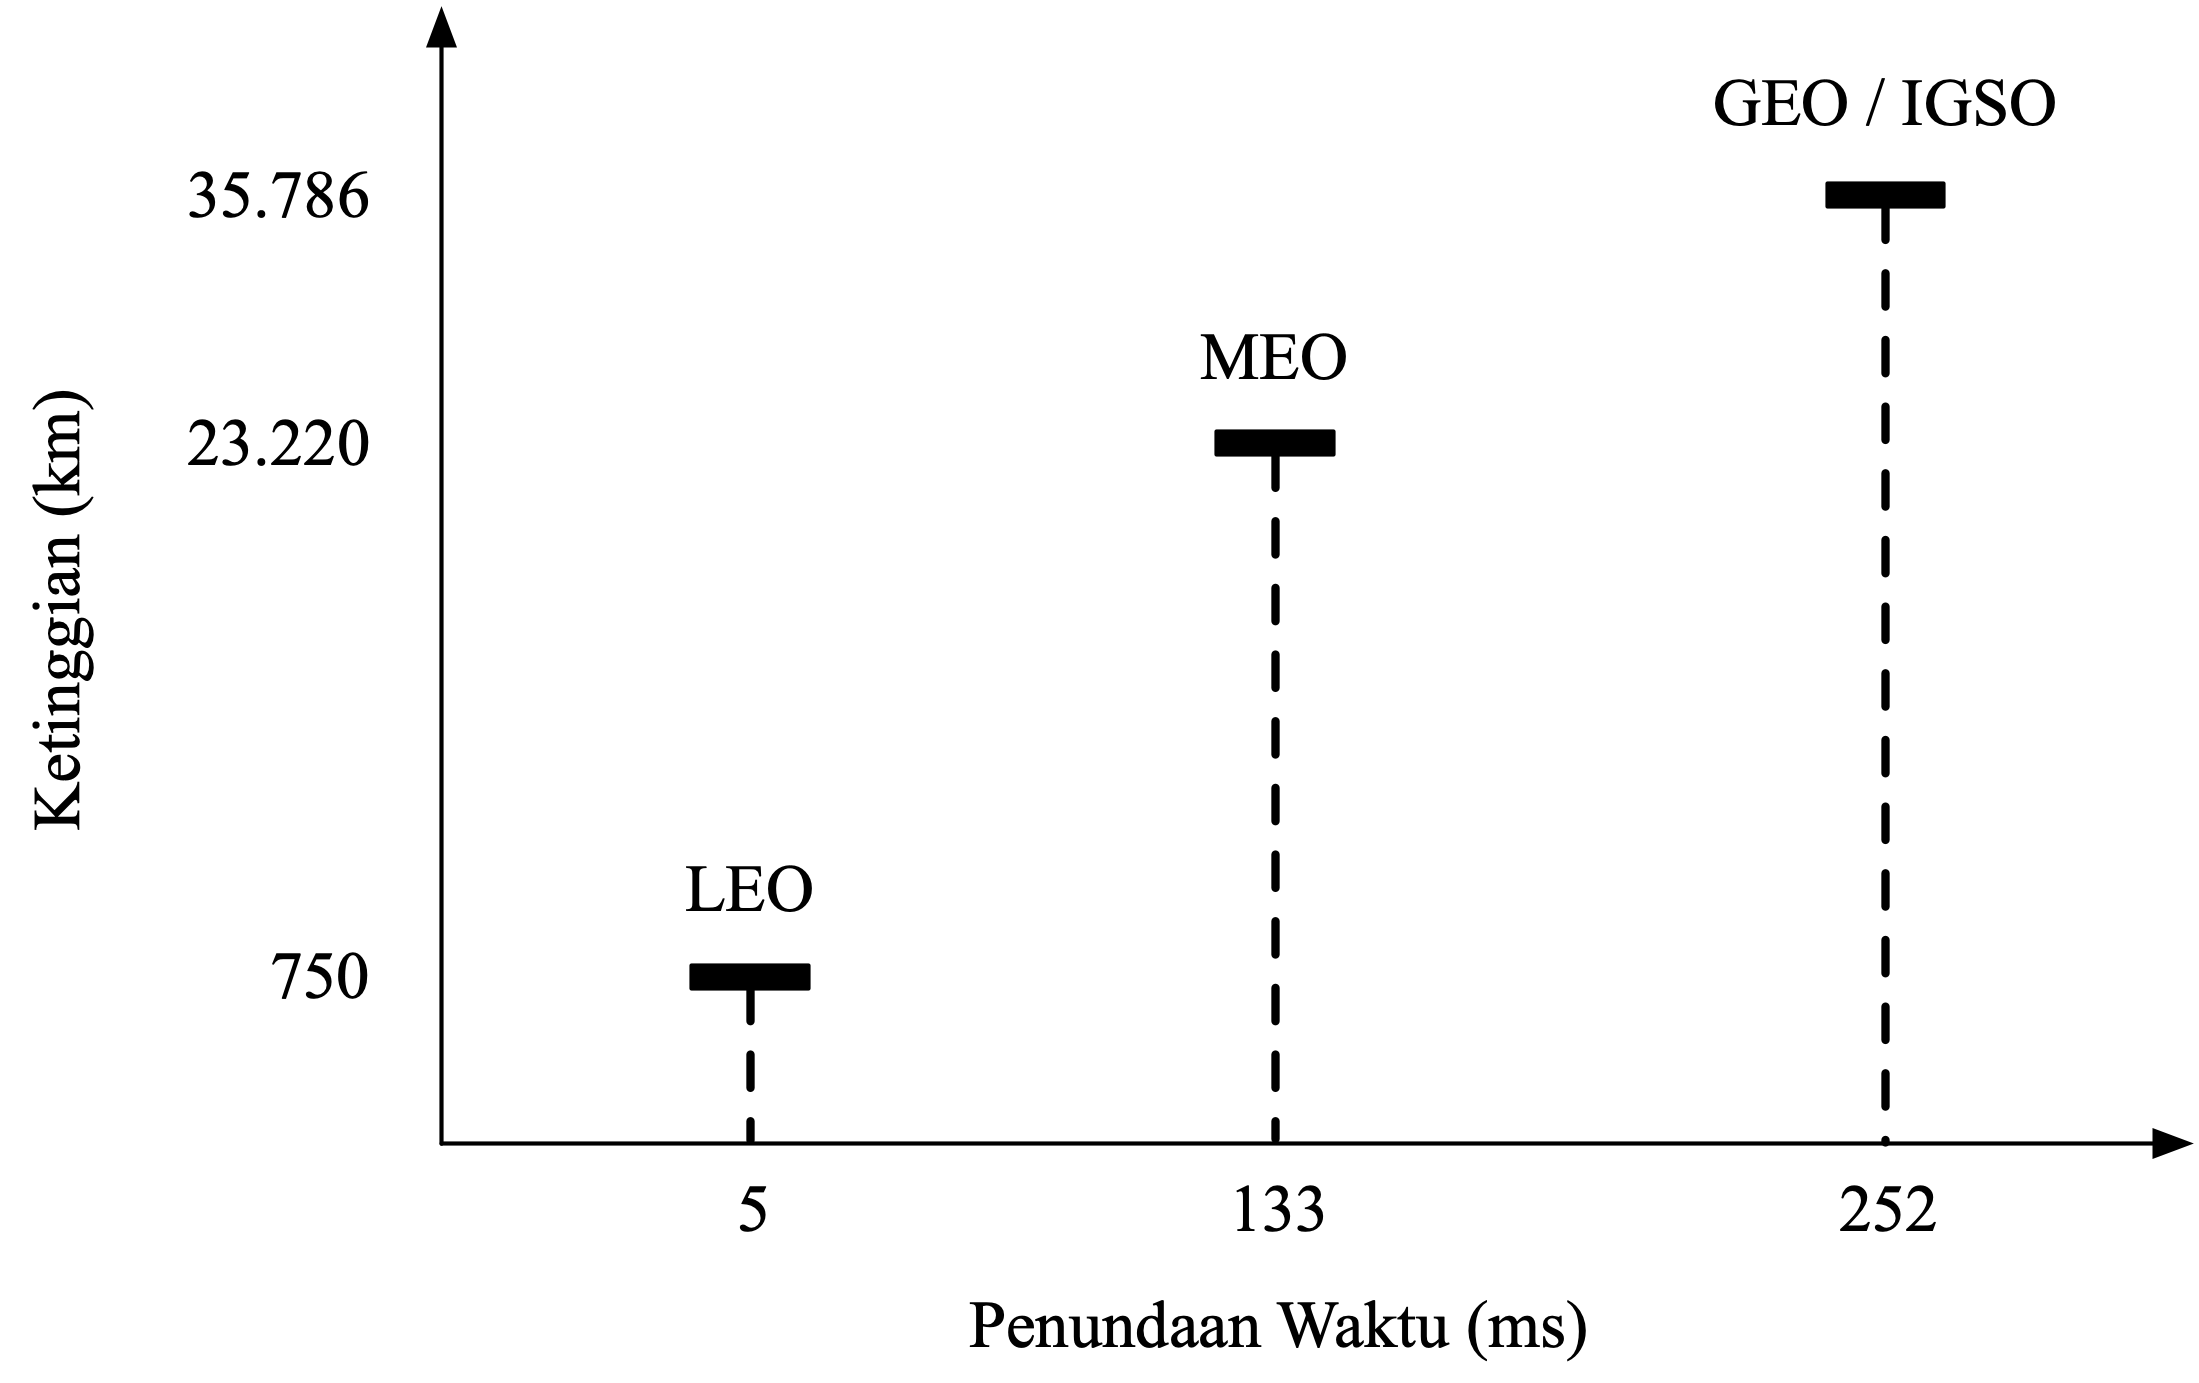
\includegraphics[width=10cm]{contents/chapter-2/alt-comp.png}
	\caption{Ilustrasi Orbit Satelit GNSS}
	\label{Fig: alt-comp}
\end{figure}


\begin{enumerate}
	\item \textit{Little} LEO adalah sistem yang beroperasi di bawah frekuensi 1 GHz dengan kapabilitas untuk aplikasi pesan dan suara.
	\item \textit{Big} LEO adalah sistem yang beroperasi pada Pita L dengan frekuensi 1.6 GHz s.d. 2.5 GHz dengan kapabilitas teleponi seperti suara, data, dan faksimili.
	\item \textit{Super} LEO adalah sistem yang beroperasi pada Pita Ka dengan frekuensi 20 GHz s.d. 30 GHz.
\end{enumerate}

\textbf{\textit{Medium Earth Orbit} (MEO)} adalah jenis satelit buatan yang mengorbit Bumi pada ketinggian antara 10.000 hingga 20.000 km di atas permukaan Bumi. Satelit MEO memiliki ciri khas orbitnya yang berada di antara orbit satelit LEO dan GEO. Keuntungan dari satelit MEO adalah jangkauannya yang cukup luas, sehingga hanya membutuhkan jumlah satelit yang relatif lebih sedikit untuk memberikan layanan seluruh dunia.

\textbf{\textit{Geosynchronous Equatorial Orbit} (GEO)} adalah satelit yang mengorbit Planet Bumi pada ketinggian 35.786 km. Pada orbit GEO, satelit disinkronisasi terhadap rotasi pada Planet Bumi pada arah yang sama. Jenis orbit ini memungkinkan untuk satelit tetap mempertahankan \textit{field of view} di atas permukaan Bumi selama dua puluh jam sehari. Keuntungan dari orbit Geo adalah secara teoretis hanya membutuhkan tiga hingga empat satelit untuk cakupan seluruh dunia. Kekurangan dari jenis orbit ini adalah biaya yang dibutuhkan lebih besar dan nilai penundaan waktunya semakin besar karena semakin jauh dari permukaan Bumi.

\subsubsection{Penerima GNSS}
Penerima GNSS adalah bagian dari segmen pengguna. Isyarat yang dikirimkan oleh satelit berisi efemeris, almanak, dan komponen lainnya seperti tanggal dan status satelit.

Gambar \ref{Fig: gnss_message_structure} menunjukan lima \textit{sub-frame} pada pesan yang diterima. Efemeris berisi informasi keadaan satelit dan posisinya pada orbit, sedangkan almanak berisi informasi yang lebih umum mengenai posisi pada orbit \cite{Lenhart2022}. Dibutuhkan waktu 12.5 menit untuk mengunduh almanak dan 18 detik untuk mengunduh efemeris. Ketika modul GNSS diaktifkan untuk pertama kali maka ia akan mengunduh data tersebut dan melakukan fiksasi terhadap tiga (2D) atau empat (3D) buah satelit. Proses tersebut dikenal sebagai \textit{cold start}. 

\begin{figure}[ht]
	\centering
	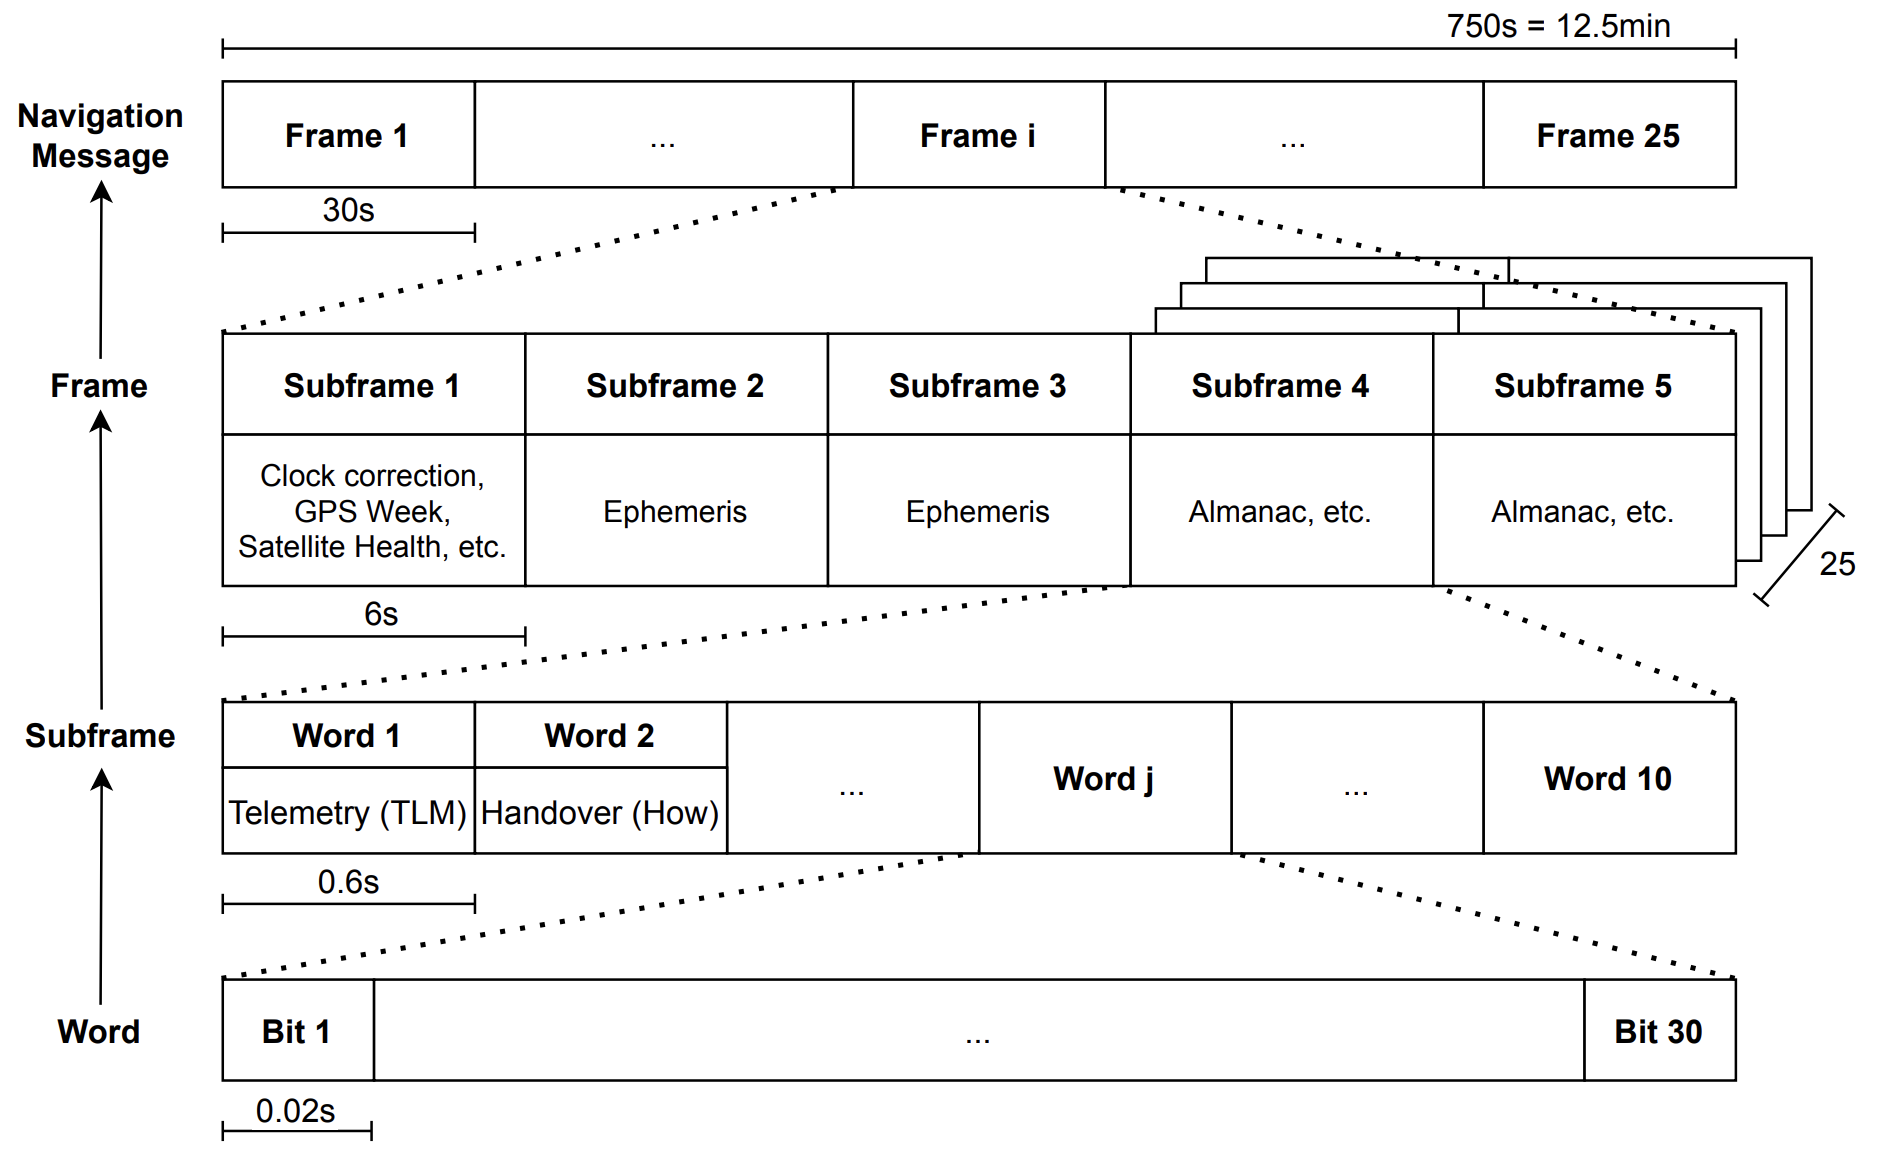
\includegraphics[width=13cm]{contents/chapter-2/gnss_msg_structure.png}
	\caption{Struktur pesan C/A NAV GNSS}
	\label{Fig: gnss_message_structure}
\end{figure}

\subsubsection{Standar NMEA 0813}
Standar NMEA 0813 adalah standar yang dimiliki oleh sebuah organisasi di Amerika Serikat dengan nama \textit{National Marine Electronics Association} sebagai wadah untuk keperluan di bidang elektronika maritim seperti pengembangan industri dan pendidikan. Organisasi ini adalah organisasi nirlaba yang dibangun oleh pelaku-pelaku pada pasar pada bidang elektronika maritim seperti manufaktur, penjual, distributor, dan institut pendidikan.

Ide dasar dari standar NMEA 0183 adalah mengirimkan data sebanyak satu baris dalam bentuk teks ASCII termasuk dengan \textit{carriage return} dan \textit{line feed} yang dikirimkan dalam \textit{baudrate} tertentu. Setiap data dikirimkan dengan kalimat yang diawali oleh simbol dollar ('\$'), dua huruf sebagai \textit{talker} ID, tiga huruf \textit{sentence} ID, data yang dipisahkan oleh tanda koma,, dan diakhiri oleh \textit{checksum} untuk integritas data. Bagian \textit{checksum} dipisahkan oleh tanda asteris ('*') dan dua digit heksadesimal yang ditunjuka dalam bentuk operasi XOR dari sluruh karakter di antara tanda dollar dan asteris.

Seiring berjalannya waktu, standar ini sudah mengalami berbagai macam revisi. Berbagai merek juga memiliki kalimat \textit{proprietary}-nya masing-masing seperti \texttt{\$PSTM} pada modul GNSS Teseo-LIV3FL yang diproduksi oleh STMicroelectronics. Standar NMEA menyajikan data-data dari modul GNSS dalam berbagai format kalimat. Beberapa contoh kalimat NMEA adalah sebagai berikut:
\begin{enumerate}
	\item \texttt{\$GPRMC} berisi data minimal yang direkomendasikan untuk disajikan oleh modul GNSS. Adapun data yang direkomendasikan adalah koordinat garis lintang dan garis bujur, ketinggian, kecepatan, dan waktu UTC.
	\item \texttt{\$GNGSA} berisi mode navigasi saat ini (2D atau 3D) dan informasi satelit yang dilacak seperti SNR, PRN, \textit{elevation}, dan \textit{azimuth}.
	\item \texttt{\$GPGGA} berisi informasi yang hampir sama dengan kalimat \textit{\$GPRMC} dengan perbedaan terdapat informasi mengenai \textit{fix} saat ini dan visibilitas satelit.
\end{enumerate}

\subsection{Lokalisasi}
Berdasarkan penelitian X, lokalisasi adalah suatu teknik untuk menghitung posisi dari suatu titik saat ini berdasarkan komunikasi antar simpul yang lokasinya telah diketahui. Posisi saat ini dihitung berdasarkan rata-rata jarak dan sudut antara dua simpul. Beberapa konsep lokalisasi adalah sebagai berikut \cite{Alrajeh2013}:

\begin{enumerate}
	\item \textbf{Laterasi} terjadi ketika jarak antar dua simpul digunakan untuk mengestimasi posisi saat ini.
	\item \textbf{Angulasi} hampir sama dengan laterasi, tetapi pada angulasi, sudut antara dua simpul digunakan untuk mengestimasi posisi saat ini.
	\item \textbf{Trilaterasi} adaqlah teknik untuk mengestimasi posisi saat ini dengan menggunakan tiga buah simpul. Pada trilaterasi, digunakan perpotongan antara tiga buah lingkaran yang akan memberikan satu titik berisi posisi saat ini.
	\item \textbf{Multilaterasi} hampir sama dengan trilaterasi, tetapi pada multilaterasi, jumlah simpul yang digunakan lebih dari empat buah.
	\item \textbf{Triangulasi} adalah teknik untuk mengestimasi posisi saat ini menggunakan sudut antara dua impul. Digunakan hukum sinus dan kosinus untuk mengestimasi posisi saat ini.
\end{enumerate}

Selain itu, lokalisasi juga dapat dibagi menjadi GNSS \textit{based} dan GNSS \textit{free}. GNSS \textit{based} adalah suatu mekanisme suatu simpul menggunakan GNSS untuk menentukan posisi saat ini. Di sisi lain, GNSS \textit{free} tidak menggunakan GNSS untuk menentukan posisi saat ini, melainkan relatif terhadap jaringan lokal.

\subsubsection{Trilaterasi}
Trilaterasi adalah proses menentukan posisi berdasarkan jarak dengan menggunakan setidaknya tiga buah satelit \cite{AmericanSocietyofCivilEngineers1994}. Ilustrasi dari trilaterasi sederhana dengan tiga buah satelit dapat dilihat pada Gambar \ref{Fig: Trilaterasi}. Misalkan titik merah, hijau, dan biru muda adalah letak dari tiga satelit dan lingkaran di sekitarnya adalah jangkauan dari masing-masing satelit pada bidang dua dimensi. Terlihat bahwa perkiraan lokasi pada objek adalah irisan dari ketiga lingkaran tersebut (titik berwarna biru tua). Perhitungan trilaterasi akan dibahas pada bagian selanjutnya \cite{Seo2012}.

\begin{figure}[H]
	\centering
	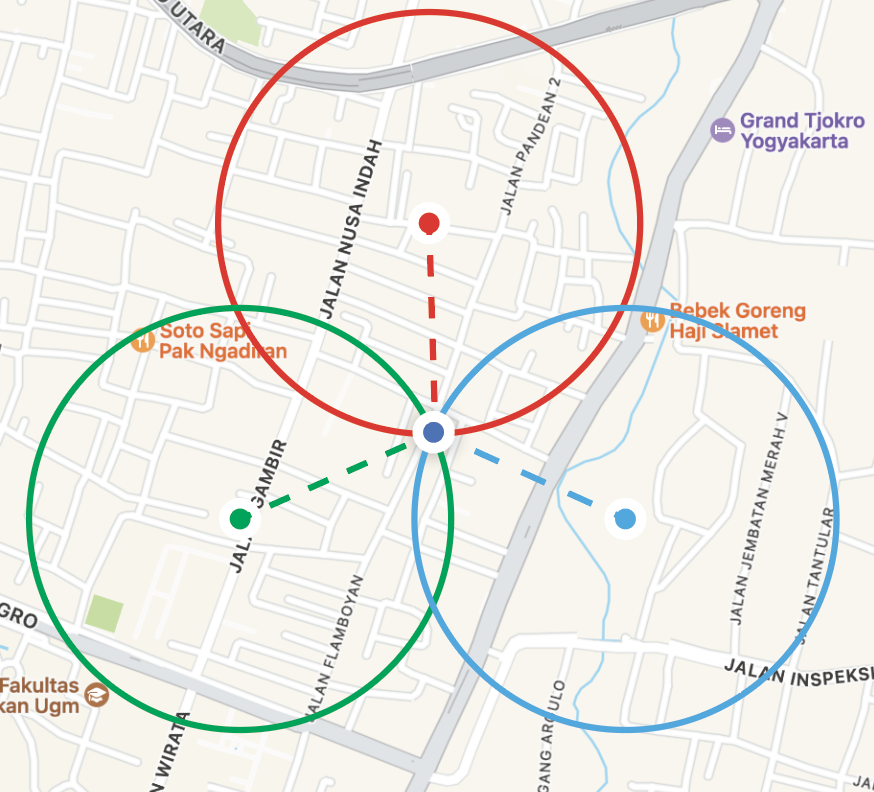
\includegraphics[width=8cm]{contents/chapter-2/trilaterasi.png}
	\caption{Trilaterasi}
	\label{Fig: Trilaterasi}
\end{figure}

Posisi objek pada bidang dua dimensi dengan Trilaterasi 2D dapat didapatkan dengan menyelesaikan tiga persamaan lingkaran yang merepresentasikan dari setiap satelit.

\begin{equation}
	\left(x-x_1\right)^2 + \left(y-y_1\right)^2=d_1^2
	\label{eq:2-1}
\end{equation}
\begin{equation}
	\left(x-x_2\right)^2 + \left(y-y_2\right)^2=d_2^2
	\label{eq:2-2}
\end{equation}
\begin{equation}
	\left(x-x_3\right)^2 + \left(y-y_3\right)^2=d_3^2
	\label{eq:2-3}
\end{equation}

Bagian kuadrat dari Persamaan \ref{eq:2-1}, \ref{eq:2-2}, dan \ref{eq:2-3} dapat diekspansikan sehingga didapat:

\begin{equation}
	x^2-2x_1x+x_1^2+y^2-2y_1y+y_1^2=d_1^2
	\label{eq:2-4}
\end{equation}
\begin{equation}
	x^2-2x_2x+x_2^2+y^2-2y_2y+y_2^2=d_2^2
	\label{eq:2-5}
\end{equation}
\begin{equation}
	x^2-2x_3x+x_3^2+y^2-2y_3y+y_3^2=d_1^2
	\label{eq:2-6}
\end{equation}

Kurangi Persamaan \ref{eq:2-5} dengan  Persamaan \ref{eq:2-4}.

\begin{equation}
	2x \left(x_2-x_1\right) + 2y \left(y_2 - y_1\right) = r_1^2 - r_2^2 - x_1^2 + x_2^2- y_1^2 + y_2^2
	\label{eq:2-7}
\end{equation}

Lakukan operasi yang sama antara Persamaan  \ref{eq:2-5} dengan Persamaan \ref{eq:2-6}.

\begin{equation}
	2x \left(x_3 -x_2\right) + 2y \left(y_3 - y_2\right) = r_2^2 - r_3^2 - x_2^2 + x_3^2- y_2^2 + y_3^2
	\label{eq:2-8}
\end{equation}

Persamaan \ref{eq:2-7} dan Persamaan \ref{eq:2-8} dapat dituliskan kembali sebagai $A$, $B$, $C$, $D$, $E$, dan $F$ seperti ditunjukan oleh Persamaan \ref{eq:2-9} dan Persamaan \ref{eq:2-10} di bawah .

\begin{equation}
	Ax + By = C
	\label{eq:2-9}
\end{equation}

\begin{equation}
	Dx + Ey = F
	\label{eq:2-10}
\end{equation}

Dua sistem persamaan linear di atas dapat ditulis kembali dalam bentuk matriks berikut:

\begin{equation}
	\begin{bmatrix}
		A & B \\
		D & E \\
	\end{bmatrix}
	\begin{bmatrix}
		x \\
		y\\
	\end{bmatrix} = 
	\begin{bmatrix}
		C \\
		F \\
	\end{bmatrix}
	\label{eq:2-11}
\end{equation}

Maka didapat solusi berupa koordinat posisi di bidang horizontal $\left(x\right)$ dan bidang vertikal $\left(y\right)$ dari sistem persamaan linear di atas.

\begin{equation}
	x = \frac{det
		\left(
			\begin{bmatrix}
				C & B \\
				F & D\\
			\end{bmatrix}
		\right)
	}{
		det\left(\
			\begin{bmatrix}
				A & B \\
				D & E\\
			\end{bmatrix}
		\right)
	}
	\label{eq:2-12}
\end{equation}

\begin{equation}
	x = \frac{det
		\left(
		\begin{bmatrix}
			A & C \\
			D & F\\
		\end{bmatrix}
		\right)
	}{
		det\left(\
		\begin{bmatrix}
			A & B \\
			D & E\\
		\end{bmatrix}
		\right)
	}
	\label{eq:2-13}
\end{equation}


\subsection{Ketelitian GNSS}
Performa modul GNSS adalah hal penting dalam aplikasi navigasi, seperti navigasi pada kendaraan udara, laut, dan darat. Modul GNSS menghasilkan informasi posisi dan waktu yang akurat berdasarkan sinyal yang diterima dari satelit. Performa modul GNSS dapat ditinjau dari tingkat akurasi dan tingkat presisinya. Akurasi mengacu pada seberapa dekat hasil pembacaan modul GNSS dengan posisi sebenarnya, sedangkan tingkat presisi menunjukkan seberapa dekat hasil yang didapat dengan rata-rata dari seluruh sampel \cite{Novatel2023}. 

Dalam aplikasi navigasi, akurasi dan presisi yang tinggi sangatlah penting. Dengan akurasi yang tinggi, pengguna dapat mengetahui posisi mereka secara tepat, sedangkan dengan presisi yang tinggi, pengguna dapat memperoleh informasi yang konsisten dan akurat meskipun dilakukan pengukuran berkali-kali pada waktu yang berbeda.

\begin{figure}[H]
	\centering
	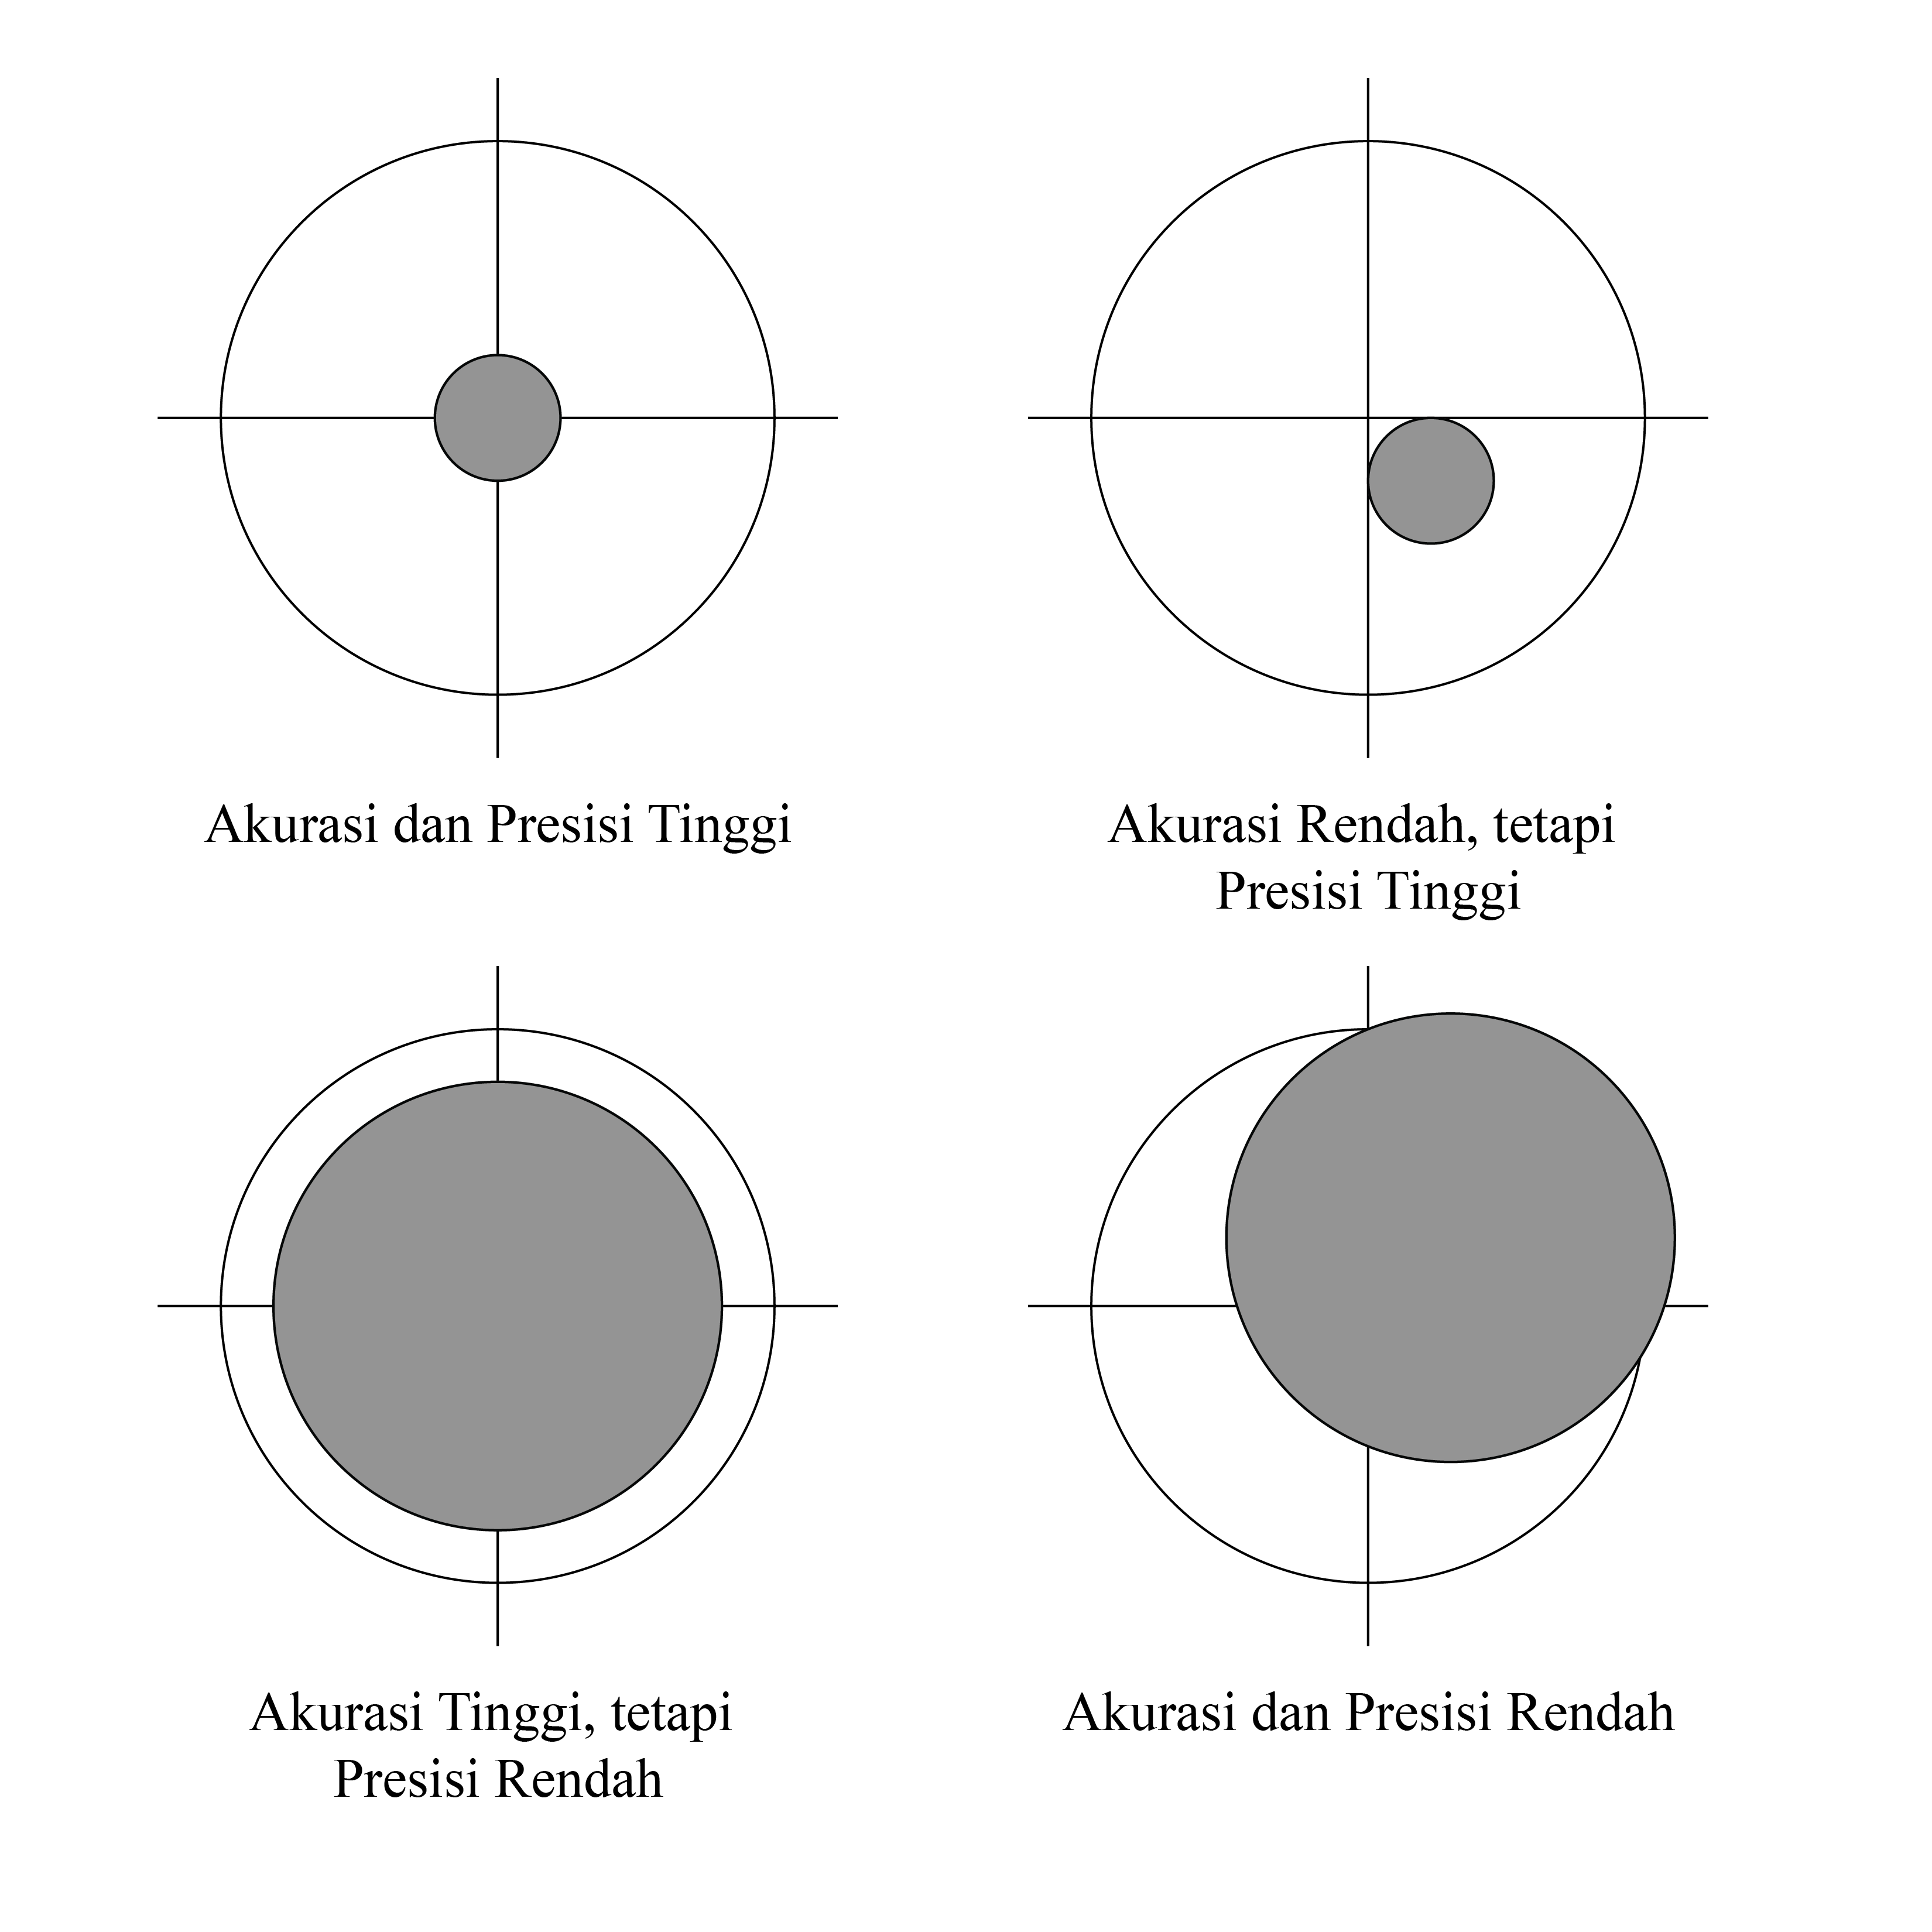
\includegraphics[width=12cm]{contents/chapter-2/acc.png}
	\caption{Ilustrasi Perbedaan Tingkat Akurasi dan Presisi}
	\label{Fig: acc-and-prec-diff}
\end{figure}

Gambar \ref{Fig: acc-and-prec-diff} adalah ilustrasi yang menjelaskan perbedaan antara tingkat akurasi dan presisi. Lingkaran dengan radius kecil tepat pada titik tengah mewakili hasil pengukuran yang memiliki tingkat akurasi dan presisi yang tinggi. Artinya, hasil pengukuran tersebut sangat dekat dengan posisi sebenarnya dan nilai rata-rata dari seluruh sampel. Lingkaran dengan radius kecil yang letaknya melenceng dari titik tengah mewakili hasil pengukuran yang memiliki tingkat akurasi yang rendah namun tingkat presisi yang tinggi. Hal ini berarti hasil pengukuran tersebut tidak dekat dengan posisi sebenarnya, namun ketika diukur berkali-kali, hasilnya akan konsisten dan akurat. Lingkaran dengan radius besar yang tepat pada titik tengah mewakili hasil pengukuran yang memiliki tingkat akurasi yang tinggi, namun presisi yang rendah. Artinya, hasil pengukuran tersebut dekat dengan posisi sebenarnya, tetapi nilai rata-rata dari seluruh sampel cukup jauh dari hasil pengukuran. Terakhir, lingkaran dengan radius besar dan melenceng dari titik tengah mewakili hasil pengukuran yang memiliki tingkat akurasi dan presisi yang rendah. Artinya, hasil pengukuran tersebut tidak dekat dengan posisi sebenarnya dan nilai rata-rata dari seluruh sampel juga cukup jauh dari hasil pengukuran.

\subsubsection{\textit{Dilution of Precision}}
\textit{Dilution of Precision} atau DOP adalah suatu konsep sederhana yang banyak digunakan untuk mengukur efektivitas dari suatu pengukuran. Nilai DOP dapat diestimasi menggunakan perhitungan yang telah dlakukan pada penelitian \cite{Tahsin2015} . Semakin kecil nilai DOP maka semakin baik \cite{Hofmann-Wellenhof2008}. Klasifikasi nilai DOP menurut \cite{Langley1999} ditunjukan oleh Tabel \ref{Tab: Nilai_DOP}.

Nilai DOP dapat dibagi menjadi tiga, yaitu
\begin{enumerate}
	\item \textbf{\textit{Horizontal Dilution of Precision} (HDOP)}: Mendeskripsikan efek dari nilai DOP pada bidang horizontal. Semakin rendah nilai HDOP maka semakin akurat posisi garis bujur dan garis lintang yang didapat.
	\item \textbf{\textit{Vertical Dilution of Precision} (VDOP)}: Mendeskripsikan efek dari nilai DOP pada posisi vertikal. Semakin rendah nilai VDOP maka semakin akurat nilai ketinggian yang didapat.
	\item \textbf{\textit{Position Dilution of Precision} (PDOP)}: Merupakan gabungan dari HDOP dan VDOP. Selain itu, PDOP juga mendeskripsikan persebaran satelit di langit. Semakin kecil nilai PDOP maka posisi satelit semakin tersebar, sehingga akurasi yang didapat semakin besar.
\end{enumerate}

\begin{table}[H]
	\caption{Klasifikasi Nilai DOP \cite{Langley1999}}
	\vspace{0.5em}
	\centering
	\begin{tabulary}{1.0\textwidth}{p{.1\textwidth} p{.2\textwidth} p{.6\textwidth} }
		\hline
		\multicolumn{1}{c}{\textbf{DOP}} & \multicolumn{1}{c}{\textbf{Klasifikasi}} & \multicolumn{1}{c}{\textbf{Keterangan}}\\
		\hline 
		
		\multicolumn{1}{c}{< 1} & 
		\multicolumn{1}{c}{Ideal} & 
		Dapat digunakan untuk aplikasi yang membutuhkan ketelitian tinggi.\\
		
		\multicolumn{1}{c}{1 - 2} & 
		\multicolumn{1}{c}{Sangat Baik} & 
		Hasil pengukuran posisi sudah cukup untuk aplikasi yang sensitif terhadap ketelitian.\\
		
		\multicolumn{1}{c}{2 - 5} & 
		\multicolumn{1}{c}{Cukup} &
		Standar minimal hasil pengukuran. \\ 
		
		\multicolumn{1}{c}{5 - 10} & 
		\multicolumn{1}{c}{Sedang} & 
		Hasil pengukuran posisi sudah dapat digunakan, tetapi kualitas \textit{fix}-nya masih harus diperbaiki.\\
		
		\multicolumn{1}{c}{10 - 20} & 
		\multicolumn{1}{c}{Buruk}  & 
		Estimasi posisi hanya dapat digunakan untuk estimasi saja.\\ 
		
		\multicolumn{1}{c}{> 20} & 
		\multicolumn{1}{c}{Sangat Buruk} & 
		Hasil pengukuran tidak dapat digunakan.
		
		\\ \hline
	\end{tabulary}
	\label{Tab: Nilai_DOP}
\end{table}

\subsubsection{\textit{Circular Error Probability} (CEP)}
\textit{Circular Error Probability} atau CEP adalah nilai yang digunakan untuk meninjau tingkat kepresisian dari suatu modul GNSS. Nilai CEP didefinisikan sebagai jari-jari dari lingkaran yang berisi 50\% dari hasil pengukuran dengan jari-jari di nilai rata-ratanya. Nilai CEP dapat dihitung dengan menggunakan Persamaan \ref{eq:CEP}.

\begin{equation}
CEP = 0.62 \sigma_y + 0.56 \sigma_x
\label{eq:CEP}
\end{equation}

dengan $\sigma_x$ adalah standar deviasi garis bujur dan $\sigma_y$ adalah standar deviasi garis lintang. Nilai CEP dapat digunakan untuk meninjau tingkat ketelitian dari modul GNSS.

CEP adalah metode yang untuk melakukan analisis data terkait dengan tingkat probabilitas tertentu dan tidak terdistorsi dengan kesalahan besar \cite{Chin1983}. Kekurangan dari CEP adalah hanya meninjau 50\% data saja dan tidak memberikan informasi apapun terkait 50\% lainnya \cite{Sathish2016}. Perlu diperhatikan bahwa nilai CEP hanya dapat digunakan jika data yang dimiliki terdistribusi normal.

\subsubsection{\textit{Mean Absolute Deviation} (MAD)}
Mean absolute deviation (MAD) adalah ukuran seberapa jauh data tersebar dari nilai rata-rata (mean) dalam sebuah kumpulan data. MAD sering digunakan sebagai alternatif yang lebih \textit{robust} terhadap deviasi standar (standard deviation) dalam analisis data, terutama ketika data tidak terdistribusi secara normal.

MAD dihitung dengan cara mengambil selisih antara setiap data dan mean, kemudian menjumlahkan nilai absolut dari selisih tersebut, dan membaginya dengan jumlah data seperti ditunjukan oleh Persamaan \ref{eq:MAD}. MAD memiliki unit yang sama dengan data, sehingga mudah untuk dipahami dan diinterpretasikan. Semakin kecil nilai MAD, semakin presisi hasil pengukuran modul GNSS.

\begin{equation}
	MAD = \frac{1}{n} \sum_{i=1}^{n} \left| x_i - m(X) \right|
	\label{eq:MAD}
\end{equation}

Dalam konteks pengukuran posisi menggunakan modul GNSS, MAD dapat digunakan untuk mengukur presisi dari data posisi yang diperoleh. Semakin kecil nilai MAD, semakin presisi data posisi tersebut. Namun, nilai MAD juga dapat dipengaruhi oleh faktor lain seperti jumlah data yang digunakan, kondisi atmosfer, dan kualitas isyarat GNSS yang diterima.

\subsection{\textit{Geofence}}
\textit{Geofence} atau batasan maya adalah suatu teknologi yang digunakan untuk memantau objek di dalam suatu area tertentu \cite{Sari2021}. Penggunaan teknologi ini semakin populer dan diterapkan pada berbagai sektor, mulai dari sektor transportasi, industri, hingga sektor keamanan. Dalam sistem geofence, jika objek yang dipantau melintasi daerah di luar batasan yang telah ditentukan, maka sistem akan mengirimkan notifikasi sebagai tanda bahwa objek tersebut berada di luar daerah yang telah ditentukan. Terdapat tiga teknik yang dapat digunakan untuk mendefinisikan area \textit{geofence} \cite{Rui2015}, yaitu:

\begin{enumerate}
	\item \textbf{Poligon}: Daerah \textit{geofence} didefinisikan pada sebuah poligon dengan verteks berupa titik-titik koordinat.
	\item \textbf{\textit{Point of Interest}}: Daerah \textit{geofence} dideskripsikan sebagai suatu lingkaran dengan jari-jari tertentu dan titik pusat lingkaran berupa suatu titik koordinat.
	\item \textbf{Rute}: Daerah \textit{geofence} berada di sekitar rute yang telah ditentukan.
\end{enumerate}

Pada teknik \textit{point of interest}, jarak antara koordinat titik pusat lingkaran ke satu titik lainnya dapat dihitung menggunakan Persamaan Haversine  \cite{Pratama2020}. Persamaan Haversine digunakan untuk menghitung jarak antara dua titik koordinat pada permukaan bola seperti Bumi. Persamaan ini sangat berguna dalam aplikasi \textit{geofence} untuk menghitung jarak objek dari titik pusat lingkaran.

\subsubsection{Persamaan Haversine}
Persamaan Haversine pertama kali diciptakan oleh Prof. James Inman pada tabun 1835 untuk persamaan astronomi \textit{nautical} dan menghitung jarak antara dua bintang. Persamaan ini adalah sebuah persamaan matematika paling penting dalam bidang Navigasi. Persamaan ini digunakan untuk menghitung jarak antara dua titik koordinat pada permukaan bola, khususnya pada Planet Bumi \cite{Hofmann-Wellenhof2008}\cite{Feng2013}. Persamaan Haversine menggunakan dua titik koordinat garis lintang dan garis bujur dari kedua titik tersebut. Jika sudut pusat antara kedua titik adalah $\theta = \frac{d}{r}$, maka fungsi Haversin dapat didefinisikan sebagai:

$$\text{hav}(\theta) = \sin^2{\left(\frac{\theta}{2}\right)}$$

Asumsikan bahwa Planet Bumi berbentuk bola sempurna dengan jari-jari $R=6.367,45$km. Selain itu, efek elipsoidal dan ketinggian juga akan diabaikan. Misalkan dua titik di permukaan bumi dengan koordinat masing-masing adalah $(lat_1, lon_1)$ dan $(lat_2, lon_2)$ dalam satuan radian. Selisih dari titik koordinat garis bujur dan garis lintangnya adalah

$$
\begin{aligned}
	\Delta lat &= lat_1 - lat_2 \\
	\Delta lon &= lon_1 - lon_2
\end{aligned}
$$

Persamaan Haversin untuk dua buah titik di permukaan suatu bola didefinisikan sebagai

$$
h = \mathrm{hav}\left(\frac{d}{R}\right) = \mathrm{hav}\left(\Delta lat\right) + \cos{\left(lat_1\right)} \cos{\left(lat_2\right)} \mathrm{hav}\left(\Delta lon\right)
$$
dengan $d$ adalah jarak dari dua titik dan $R$ adalah jari-jari dari bola.

Maka jarak $d$ dari kedua titik tersebut didapat dengan mengalikan jari-jari Planet Bumi $r$ dengan invers dari fungsi Haversin \cite{Omatu2013}

$$
\begin{aligned}
	d &= r \text{ }\mathrm{archav}(h) = 2r \arcsin{\left(\sqrt{h}\right)} \\
	&= 2r \arcsin{\sqrt{\sin^2{\left(\frac{\Delta lat}{2}\right)}  \cos{(lat_1)}\cos{(lat_2)} +\sin^2{\left(\frac{\Delta lon}{2}\right)}}}
\end{aligned} 
$$

Metode komputasi menggunakan Persamaan Haversine terbukti lebih sederhana dan ringan dibandingkan dengan Metode Vincenty, dengan persentase galat yang sangat kecil, yaitu 0-0,334\% \cite{Mahmoud2016}. Dalam dunia navigasi, Persamaan Haversine memiliki peran yang sangat penting dalam menghitung jarak antara dua titik koordinat pada permukaan bola.

\subsection{STM32}
STM32 adalah salah satu jenis mikrokontroler 32-bit yang sangat populer di industri saat ini. Dikembangkan oleh perusahaan teknologi STMicroelectronics, STM32 merupakan mikrokontroler berbasis arsitektur ARM Cortex-M yang memiliki performa tinggi dan konsumsi daya yang rendah. Keluarga mikrokontroler STM32 dapat dibagi menjadi lima kelompok, yaitu \textit{Mainstream}, \textit{High Performance}, \textit{Ultra-low-power}, dan \textit{Wireless}. Setiap kelompok ditujukan untuk aplikasi yang berbeda-beda dengan kebutuhan yang berbeda pula. Pembagian kelompok mikrokontroler STM32 dapat dilihat pada Gambar \ref{Fig: stm32-groups}.

\begin{figure}[H]
	\centering
	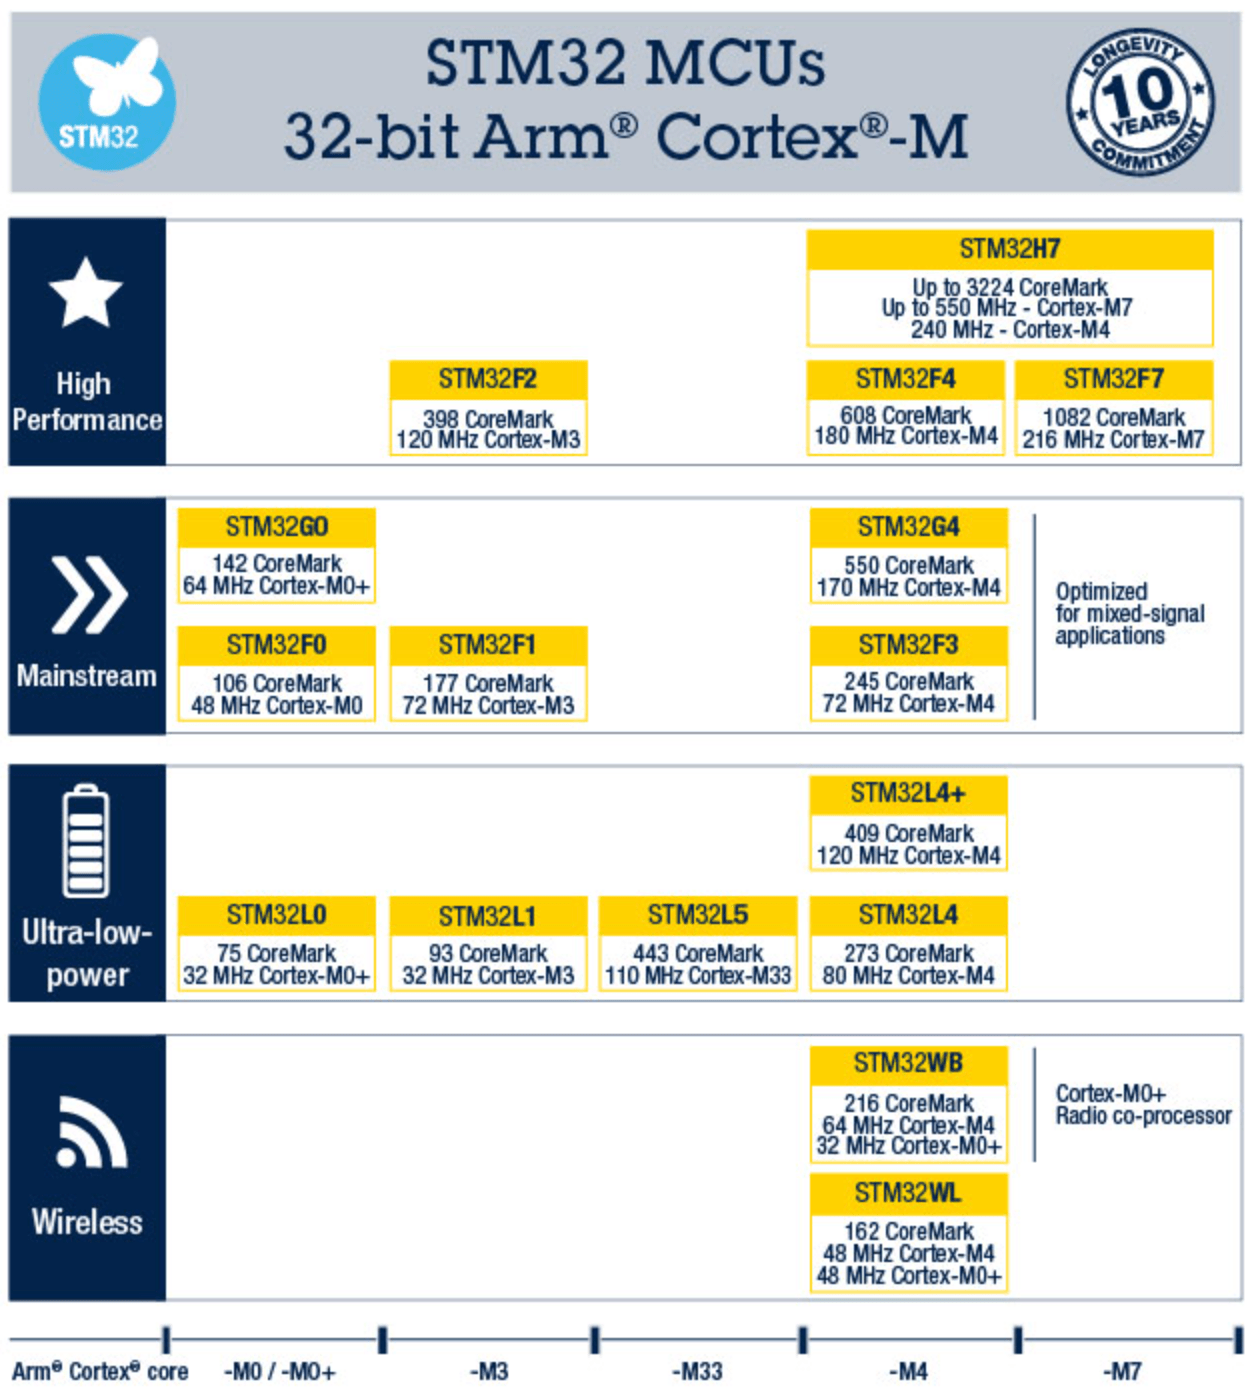
\includegraphics[width=11cm]{contents/chapter-2/stm-32-groups.png}
	\caption{Pembagian Mikrokontroler STM32 \cite{STMicroelectronics2023}}
	\label{Fig: stm32-groups}
\end{figure}

Tabel \ref{Tab: stm-arch-table} menunjukkan jenis arsitektur yang digunakan oleh setiap seri mikrokontroler STM32. Saat ini, STM32 menggunakan enam jenis arsitektur ARM Cortex yang berbeda-beda. Setiap seri mikrokontroler STM32 menggunakan arsitektur tertentu yang dipilih berdasarkan kebutuhan aplikasi yang dituju. Sebagai contoh, seri STM32 F4, F7, dan H7 menggunakan arsitektur Cortex-M7F yang menawarkan performa tinggi dengan kecepatan clock hingga 480 MHz.

\begin{table}[H]
	\caption{Jenis STM32 dan Arsitekturnya}
	\vspace{0.5em}
	\centering
	\begin{tabular}{cc}
		\hline
		\textbf{Arsitektur} & \textbf{Seri STM32} \\
		\hline 
		Cortex-M3 & F1, F2, dan L1\\
		Cortex-M4F & F3, F4, G4, L4, L4+, WB, dan WL\\
		Cortex-M0 & F0\\ 
		Cortex-M0+ & G0 dan L0\\
		Cortex-M7F & F7 dan H7\\ 
		Cortex-M33F & L5 dan U5\\ \hline
	\end{tabular}
	\label{Tab: stm-arch-table}
\end{table}

Salah satu \textit{development board} yang menggunakan mikrokontroler STM32 adalah STM32 Nucleo-WL55JC1. Papan pengembangan ini dirancang untuk memudahkan pengembang dalam membuat prototipe aplikasi wireless dengan menggunakan mikrokontroler STM32WL55. Mikrokontroler ini merupakan versi \textit{dual-core} dari STM32 yang menggabungkan arsitektur Arm Cortex-M4 dan M0+ dengan kecepatan clock hingga 48 MHz.

\subsubsection{STM32 Nucleo-WL55JC1}
STM32 Nucleo-WL55JC1 adalah sebuah \textit{development board} yang menggunakan mikrokontroler STM32WL55 yang dikembangkan oleh ST Microelectronics. Mikrokontroler yang digunakan pada papan ini adalah STM32WL55 \textit{dual-core} Arm Cortex-M4/M0+ dengan kecepatan clock sebesar 48 MHz \cite{STMicroelectronics2022}.

\begin{figure}[ht]
	\centering
	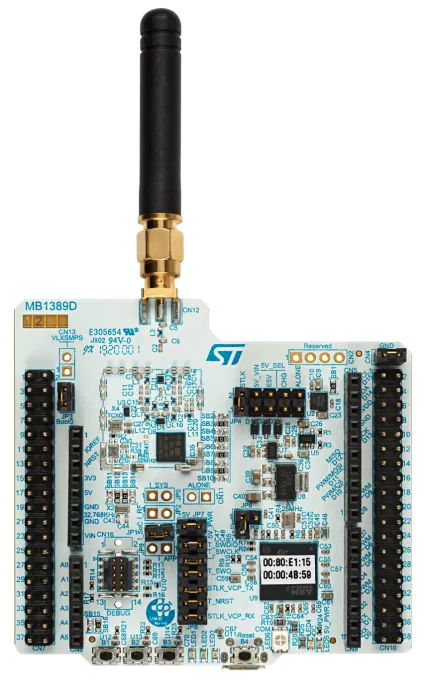
\includegraphics[width=5cm]{contents/chapter-2/stm32-wl55jc1.jpg}
	\caption{\textit{Development board} STM32 Nucleo-WL55JC1}
	\label{Fig: STM32 Nucleo-WL55JC1}
\end{figure}

Keunggulan dari \textit{development board} ini adalah sudah dilengkapi dengan STLINK-V3E yang terintegrasi, sehingga tidak memerlukan perangkat tambahan untuk melakukan pemrograman dan \textit{debugging} pada perangkat \cite{STMicroelectronics2022}. Selain itu, \textit{development board} ini juga mendukung penggunaan \textit{expansion board} Arduino dan ST morpho. Tampilan papan pengembangan STM32 Nucleo-WL55JC1 dapat dilihat pada Gambar \ref{Fig: STM32 Nucleo-WL55JC1}.

Mikrokontroler STM32WL55 memiliki kecepatan clock yang lebih cepat dibandingkan dengan kecepatan clock pada Arduino Mega yang hanya sebesar 16 MHz. Selain itu, STM32WL55 juga memiliki SRAM dengan kapasitas yang lebih besar, yaitu sebesar 64 KB atau delapan kali lipat lebih besar daripada kapasitas SRAM pada Arduino Mega \cite{STMicroelectronics2022b}.

Selain itu, komunitas pengguna STM32 juga tidak kalah besar dibandingkan dengan komunitas pengguna Arduino dan ESP-32. Hal ini menunjukkan bahwa penggunaan papan pengembangan STM32 Nucleo-WL55JC1 dapat memberikan keuntungan bagi para pengembang yang ingin menggunakan mikrokontroler dengan performa tinggi dan dukungan komunitas yang besar.

\subsubsection{STLINK-V3}
STLINK-V3 adalah perangkat yang digunakan untuk memrogram dan \textit{debugging} pada mikrokontroler STM32 dan STM8. Modul STLINK-V3 menggunakan antarmuka JTAG atau \textit{Serial Wire Debugging} (SWD) untuk melakukan komunikasi dengan mikrokontroler. Pada STM32 Nucleo-WL55JC1, STLINK-V3 sudah tertanam di \textit{development board}. Gambar \ref{Fig: stlink-in-wl55} menunjukan letak STLINK-V3 di \textit{development board} STM32 Nucleo-WL55JC1 (ditandai oleh kotak berwarna merah).

\begin{figure}[ht]
	\centering
	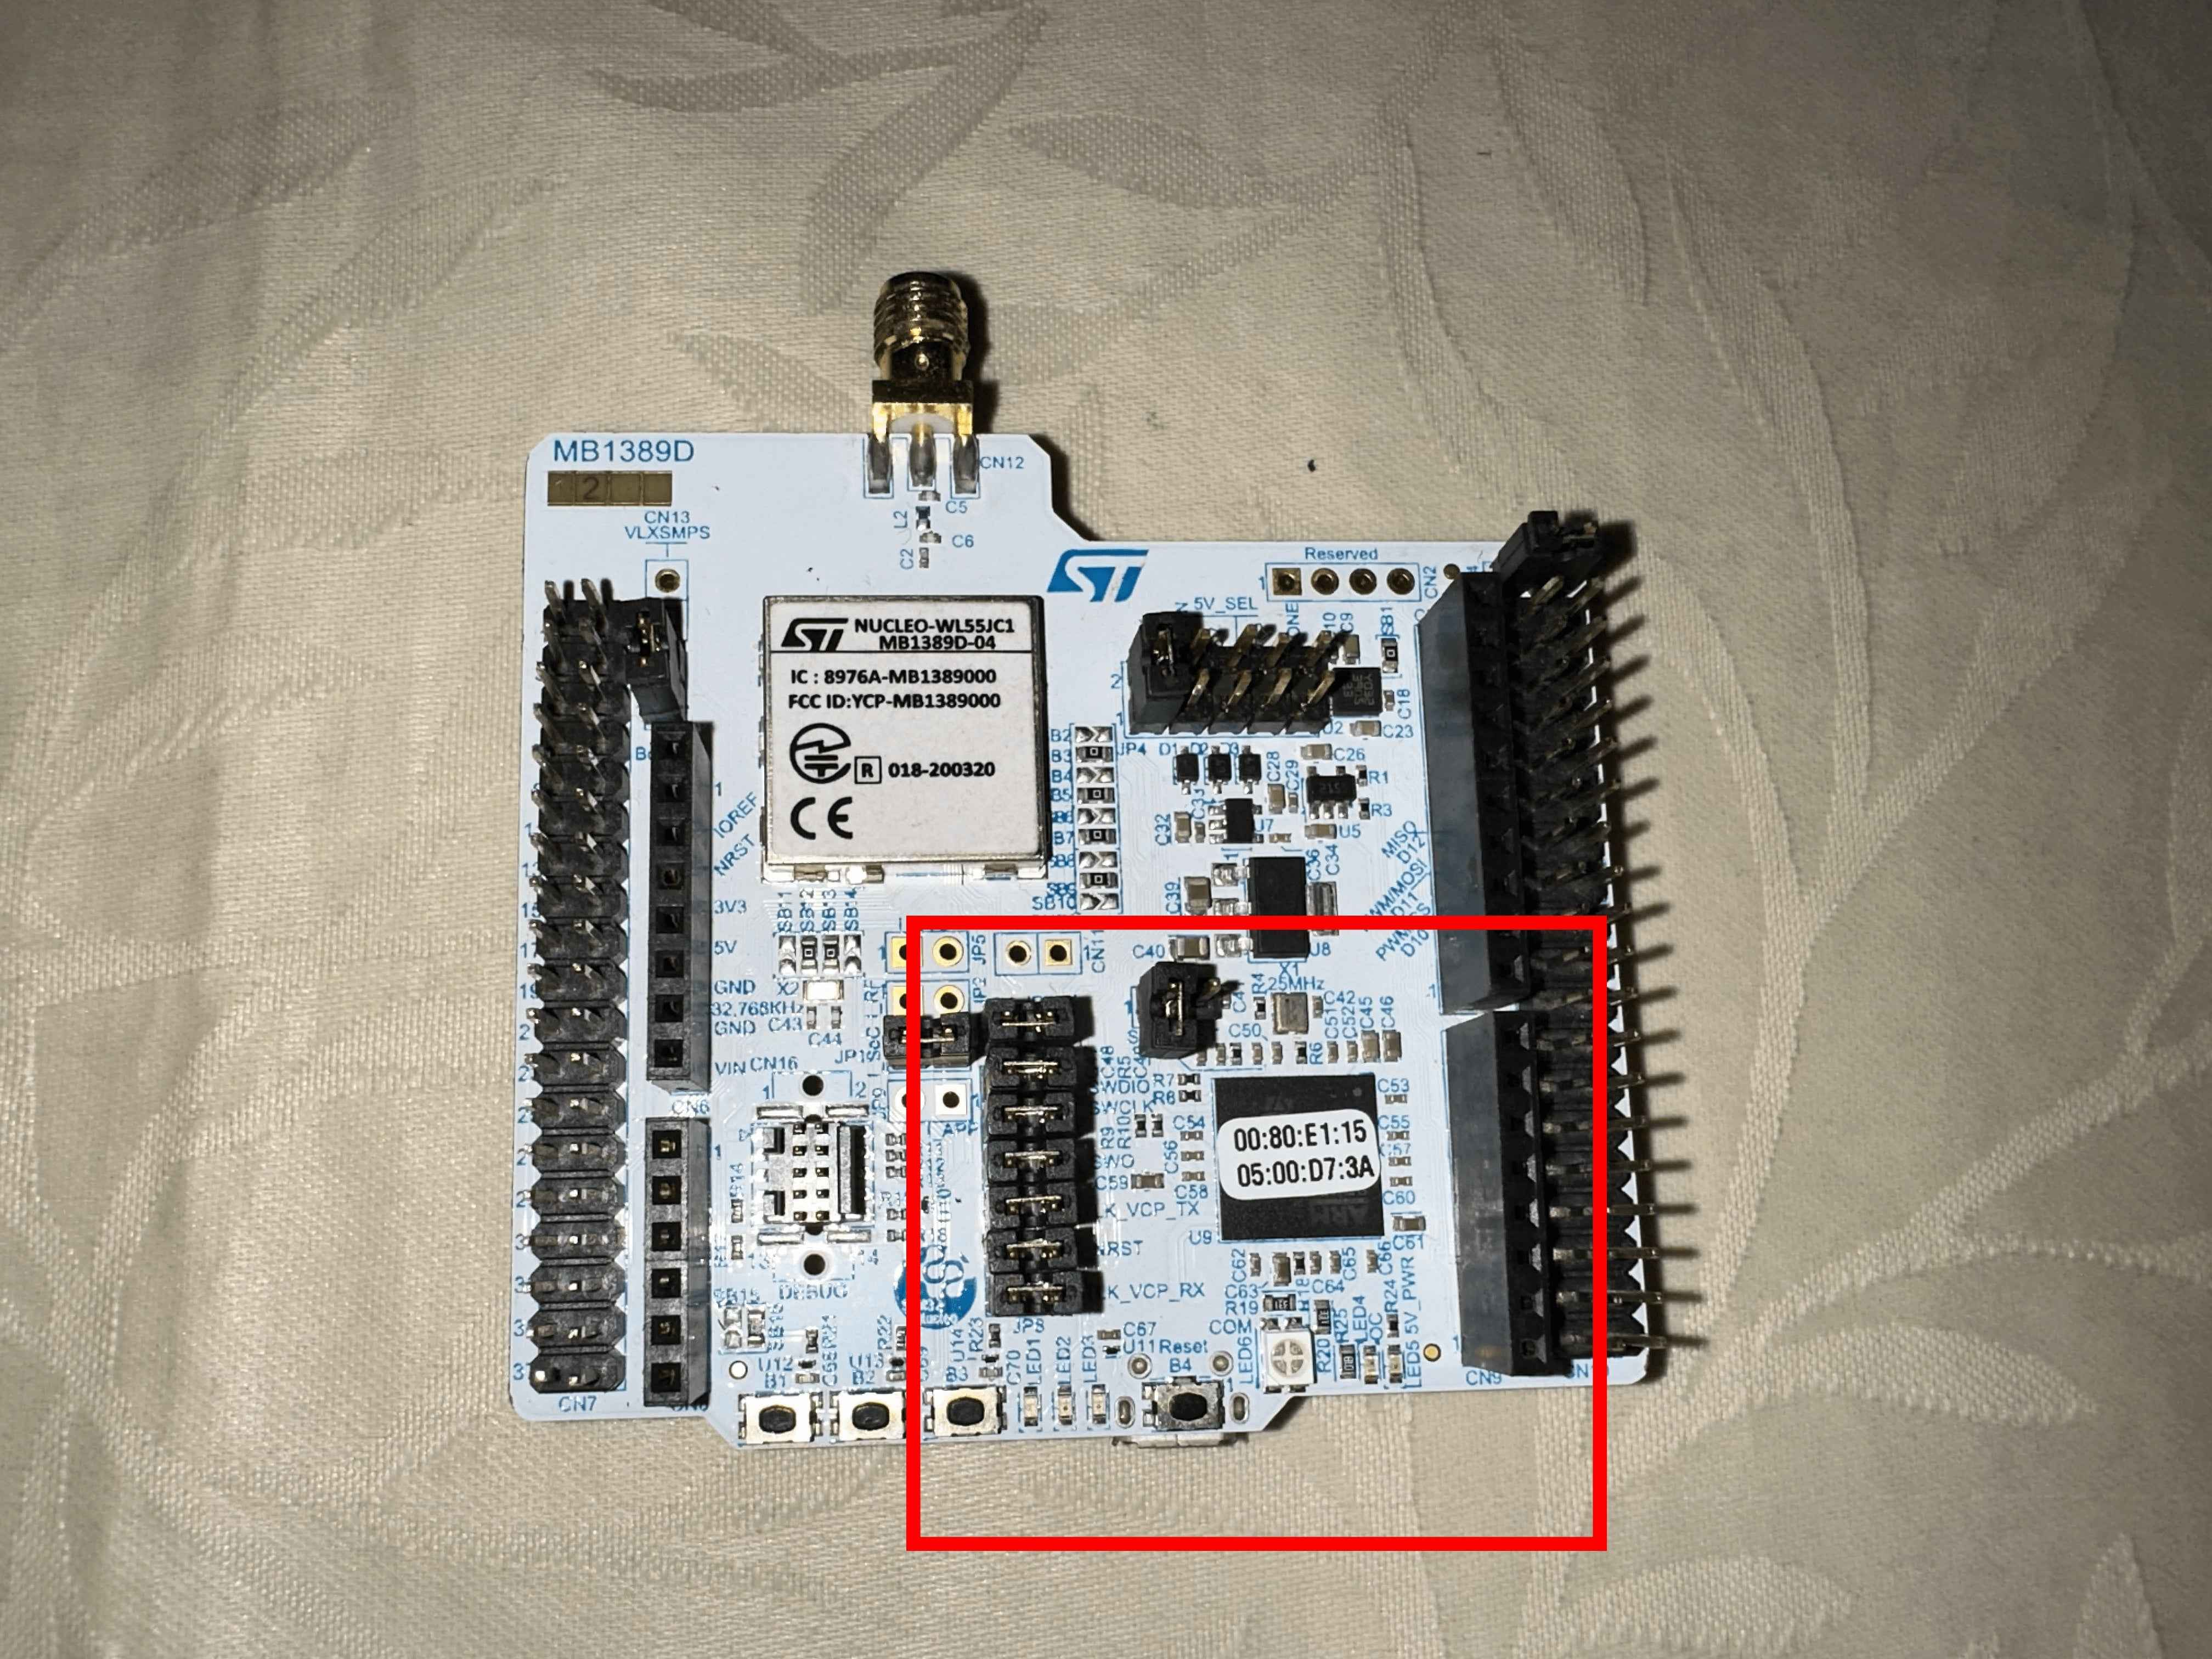
\includegraphics[width=10cm]{contents/chapter-2/stlink-in-wl55.jpg}
	\caption{Letak STLINK-V3 pada STM32 Nucleo-WL55JC1}
	\label{Fig: stlink-in-wl55}
\end{figure}

STLINK-V3 dilengkapi dengan antarmuka USB 2.0 untuk melakukan \textit{software debugging} atau pemrograman dengan menggunakan aplikasi STM32Cube IDE. Perangkat ini juga dapat digunakan untuk meninjau isyarat pada mikrokontroler dengan menggunakan fitur \textit{debug}. Beberapa fitur pada STLINK-V3 adalah \cite{STMicroelectronics2023a}:

\begin{enumerate}
	\item Mode \textit{Serial Wire Output} (SWO) dengan kecepatan 16 MHz.
	\item Mode \textit{debug} JTAG atau SWD.
	\item Komunikasi UART dengan antarmuka USB.
	\item Pemaharuan \textit{firmware} dan konfigurasi dengan aplikasi STLINK \textit{Utility}.
	\item Pengukuran profil sistem dengan \textit{energy profiling}.
\end{enumerate}

\subsubsection{STM32Cube IDE}
STM32Cube IDE merupakan sebuah \textit{platform} yang digunakan untuk pengembangan \textit{firmware} pada mikrokontroler STM32 dengan menggunakan bahasa pemrograman C/C++. Dalam STM32Cube IDE terdapat beberapa aplikasi yang dapat digunakan untuk melakukan konfigurasi periferal, menyediakan kerangka kode, \textit{compiler}, dan fitur untuk \textit{debugging} yang dapat memudahkan pengguna dalam melakukan pengembangan \textit{firmware}. Selain itu, STM32Cube IDE juga dilengkapi dengan berbagai pustaka yang dapat mendukung pengembangan dalam berbagai aplikasi.

\begin{figure}[H]
	\centering
	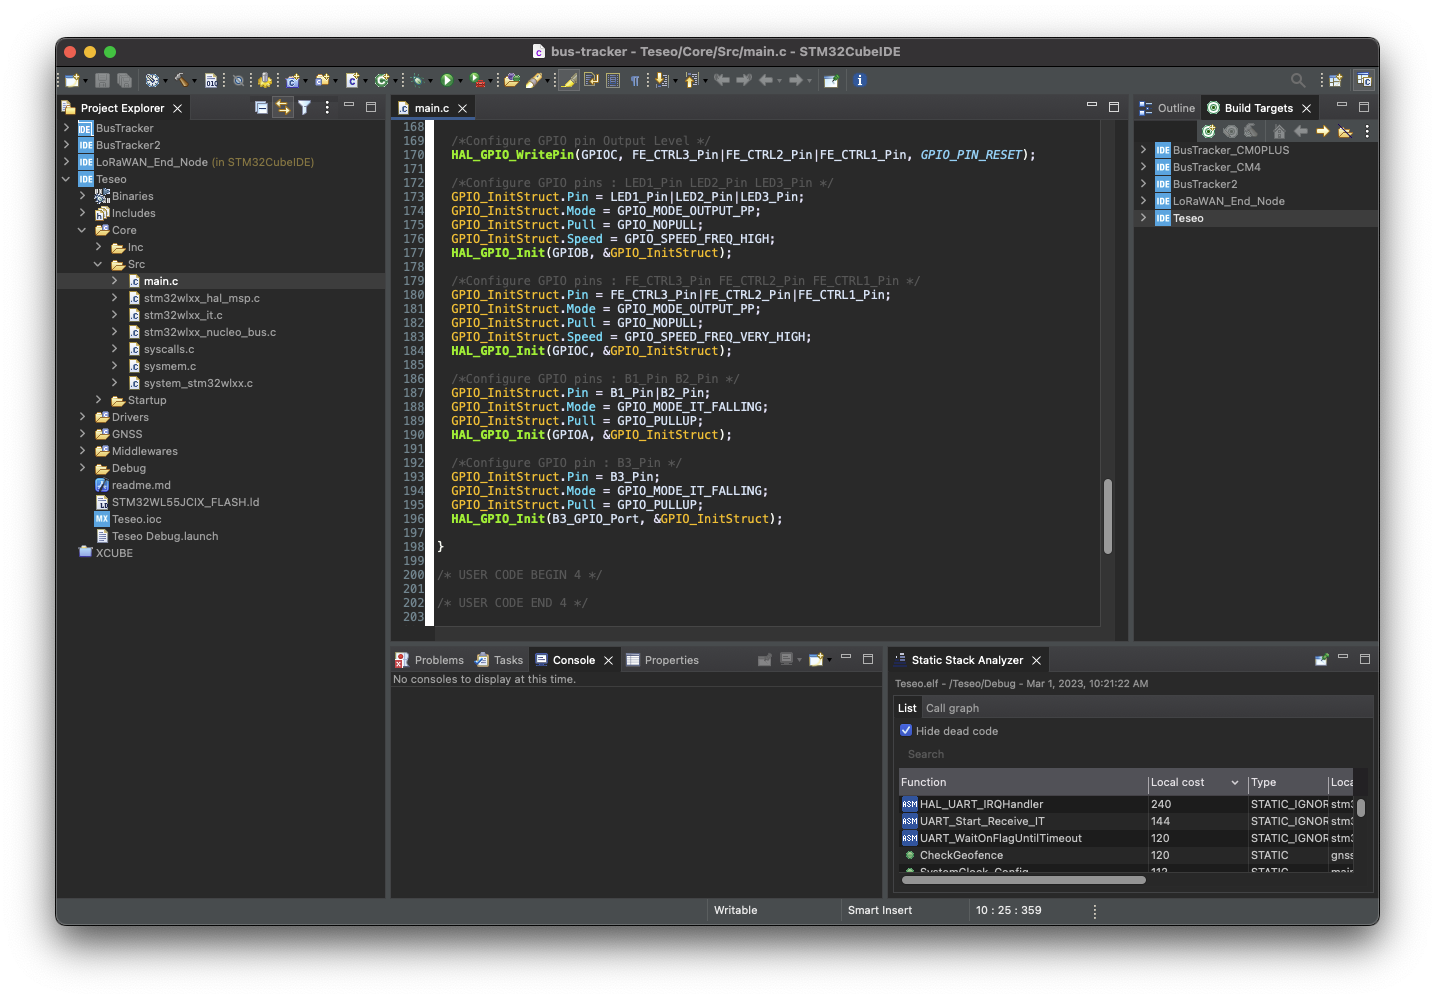
\includegraphics[width=12cm]{contents/chapter-2/stm32-ide.png}
	\caption{Tampilan STM32Cube IDE}
	\label{Fig: stm32-ide}
\end{figure}

Konfigurasi periferal pada STM32Cube IDE berbasis dari STM32Cube MX, yang merupakan perangkat lunak yang digunakan untuk mempermudah dalam melakukan konfigurasi pada mikrokontroler STM32. Tampilan dari bagian konfigurasi periferal ditunjukan oleh Gambar \ref{Fig: stm32-mx}. Konfigurasi tersebut akan disimpan dalam berkas dengan ekstensi \textit{ioc}. File \textit{ioc} dapat digunakan untuk \textit{generate} kerangka kerja yang siap untuk digunakan sehingga pengguna hanya perlu memikirkan pada sisi aplikasinya saja.

\begin{figure}[H]
	\centering
	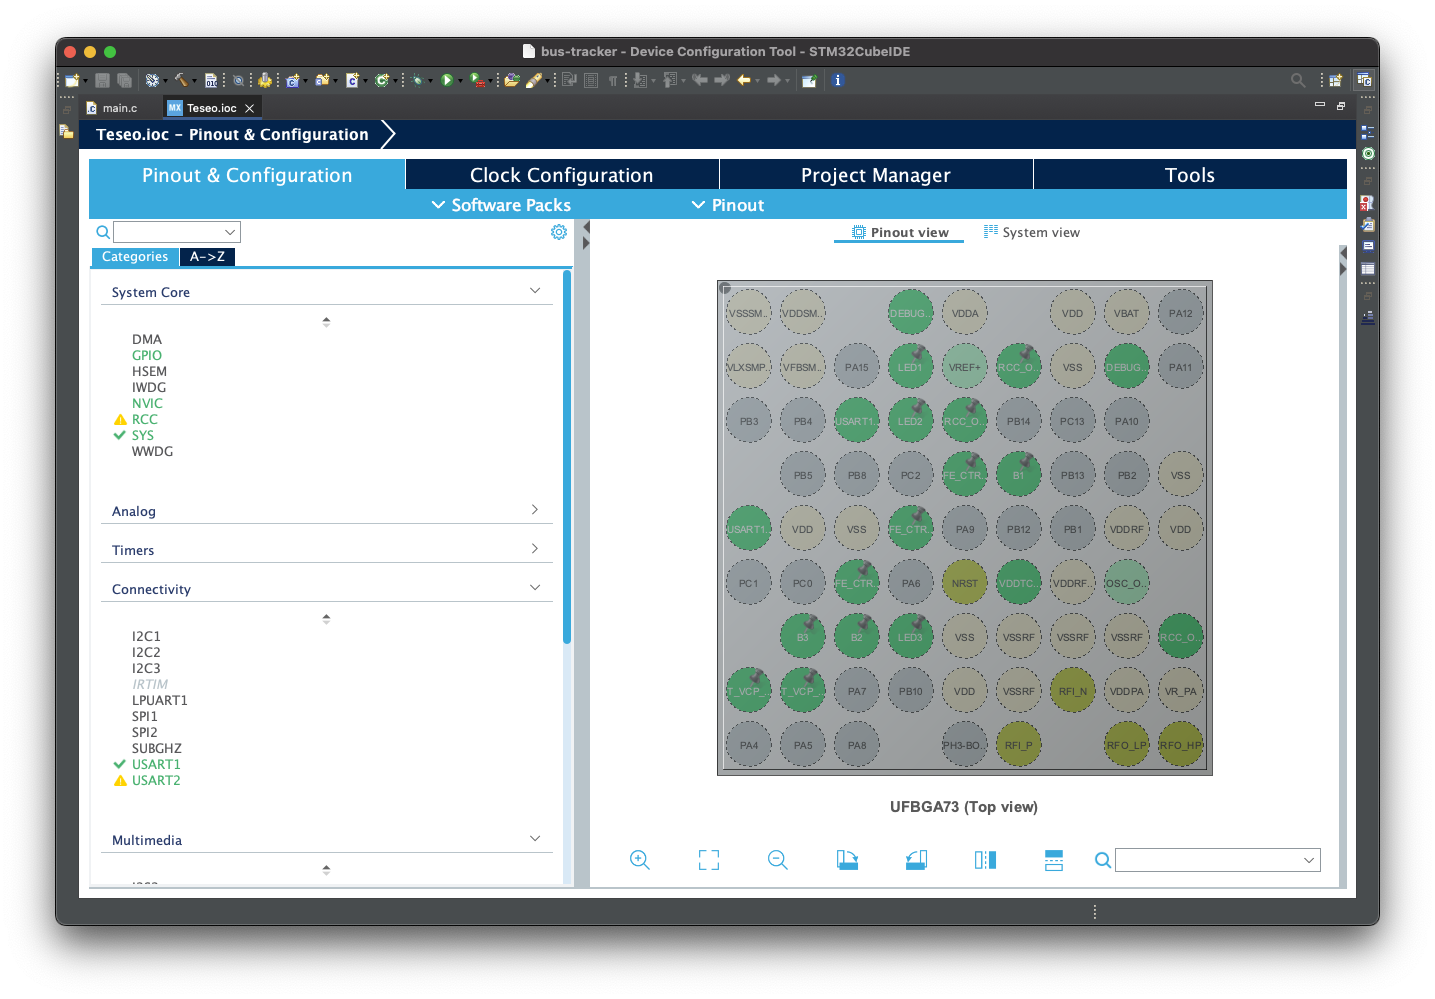
\includegraphics[width=12cm]{contents/chapter-2/stm32-mx.png}
	\caption{Konfigurasi Periferal pada STM32Cube IDE}
	\label{Fig: stm32-mx}
\end{figure}

Dalam pengembangan \textit{firmware} pada mikrokontroler STM32, STM32Cube IDE dapat membantu pengguna untuk memudahkan pengembangan \textit{firmware} dengan menggunakan berbagai alat pengembangan yang lengkap dan pustaka perangkat lunak yang lengkap sebagai referensi. Sehingga, STM32Cube IDE menjadi pilihan yang tepat bagi pengguna yang ingin melakukan pengembangan \textit{firmware} pada mikrokontroler STM32.

\subsection{Teseo-LIV3FL}
Teseo-LIV3FL adalah modul GNSS yang sangat efisien dan dapat diandalkan. Diproduksi oleh STMicroelectronics, modul ini menawarkan dukungan untuk berbagai konstelasi seperti GPS, GLONASS, Galileo, QZSS, dan BeiDou \cite{STMicroelectronics2022}. Ukuran dari modul ini adalah 9.7 x 10.1 mm dengan osilator RTC yang dapat mengurangi TTFF, menjadikannya ideal untuk aplikasi yang memerlukan respons cepat dan akurasi yang tinggi.

Untuk mengoperasikan modul Teseo-LIV3FL, dibutuhkan tegangan sebesar 3.3 V. Antarmuka UART pada modul ini memungkinkan pengguna untuk berkomunikasi dengan perangkat lain seperti mikrokontroler. Selain itu, modul ini juga dilengkapi dengan fitur \textit{anti-jamming} yang sangat berguna untuk mengurangi interferensi yang mungkin terjadi, seperti \textit{jamming} atau isyarat radio.

\begin{figure}[H]
	\centering
	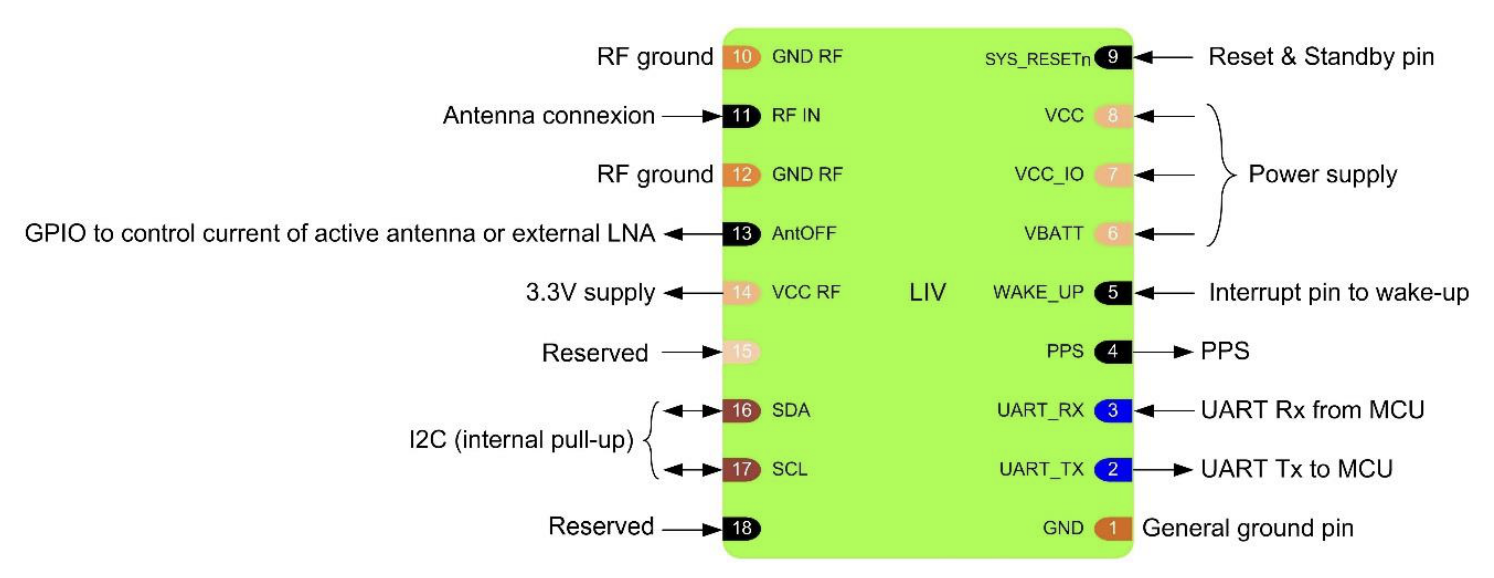
\includegraphics[width=13cm]{contents/chapter-2/teseo_pinout.png}
	\caption{\textit{Pinout} Teseo-LIV3FL \cite{STMicroelectronics2022}}
	\label{Fig: teseo_pinout}
\end{figure}

Keping GNSS Teseo-III pada modul ini memungkinkan modul ini untuk beroperasi dengan akurasi tinggi, tetapi tetap mempertahankan akurasinya. Modul Teseo-LIV3FL dapat dioperasikan dengan efisien dan hemat energi, karena hanya membutuhkan daya rendah yaitu 8$\mu$A pada mode standby dan 45mA pada mode akuisisi.

Salah satu keunggulan modul Teseo-LIV3FL adalah kustomisasi yang sangat luas. Pengguna dapat memodifikasi pengaturan modul GNSS melalui serial port atau dengan bantuan aplikasi Teeo-Suite. Hal ini memungkinkan pengguna untuk menyesuaikan modul GNSS sesuai dengan kebutuhan mereka.

\subsubsection{Teseo-Suite}
Teseo-Suite adalah aplikasi yang dikembangkan khusus untuk mengatur dan memanfaatkan fitur yang terdapat pada perangkat GNSS Teseo buatan STMicroelectronics. Aplikasi ini memiliki kemampuan untuk membaca, menyunting, dan menyimpan konfigurasi pada perangkat GNSS Teseo dengan mudah dan cepat. Dalam pengaturan konfigurasi, Teseo-Suite dapat mengatur berbagai parameter seperti pemilihan satelit, algoritma daya rendah, konfigurasi CDB-ID, dan sebagainya. Dengan fitur ini, pengguna dapat melakukan konfigurasi secara efisien dan akurat untuk memaksimalkan kinerja perangkat GNSS Teseo.

\begin{figure}[H]
	\centering
	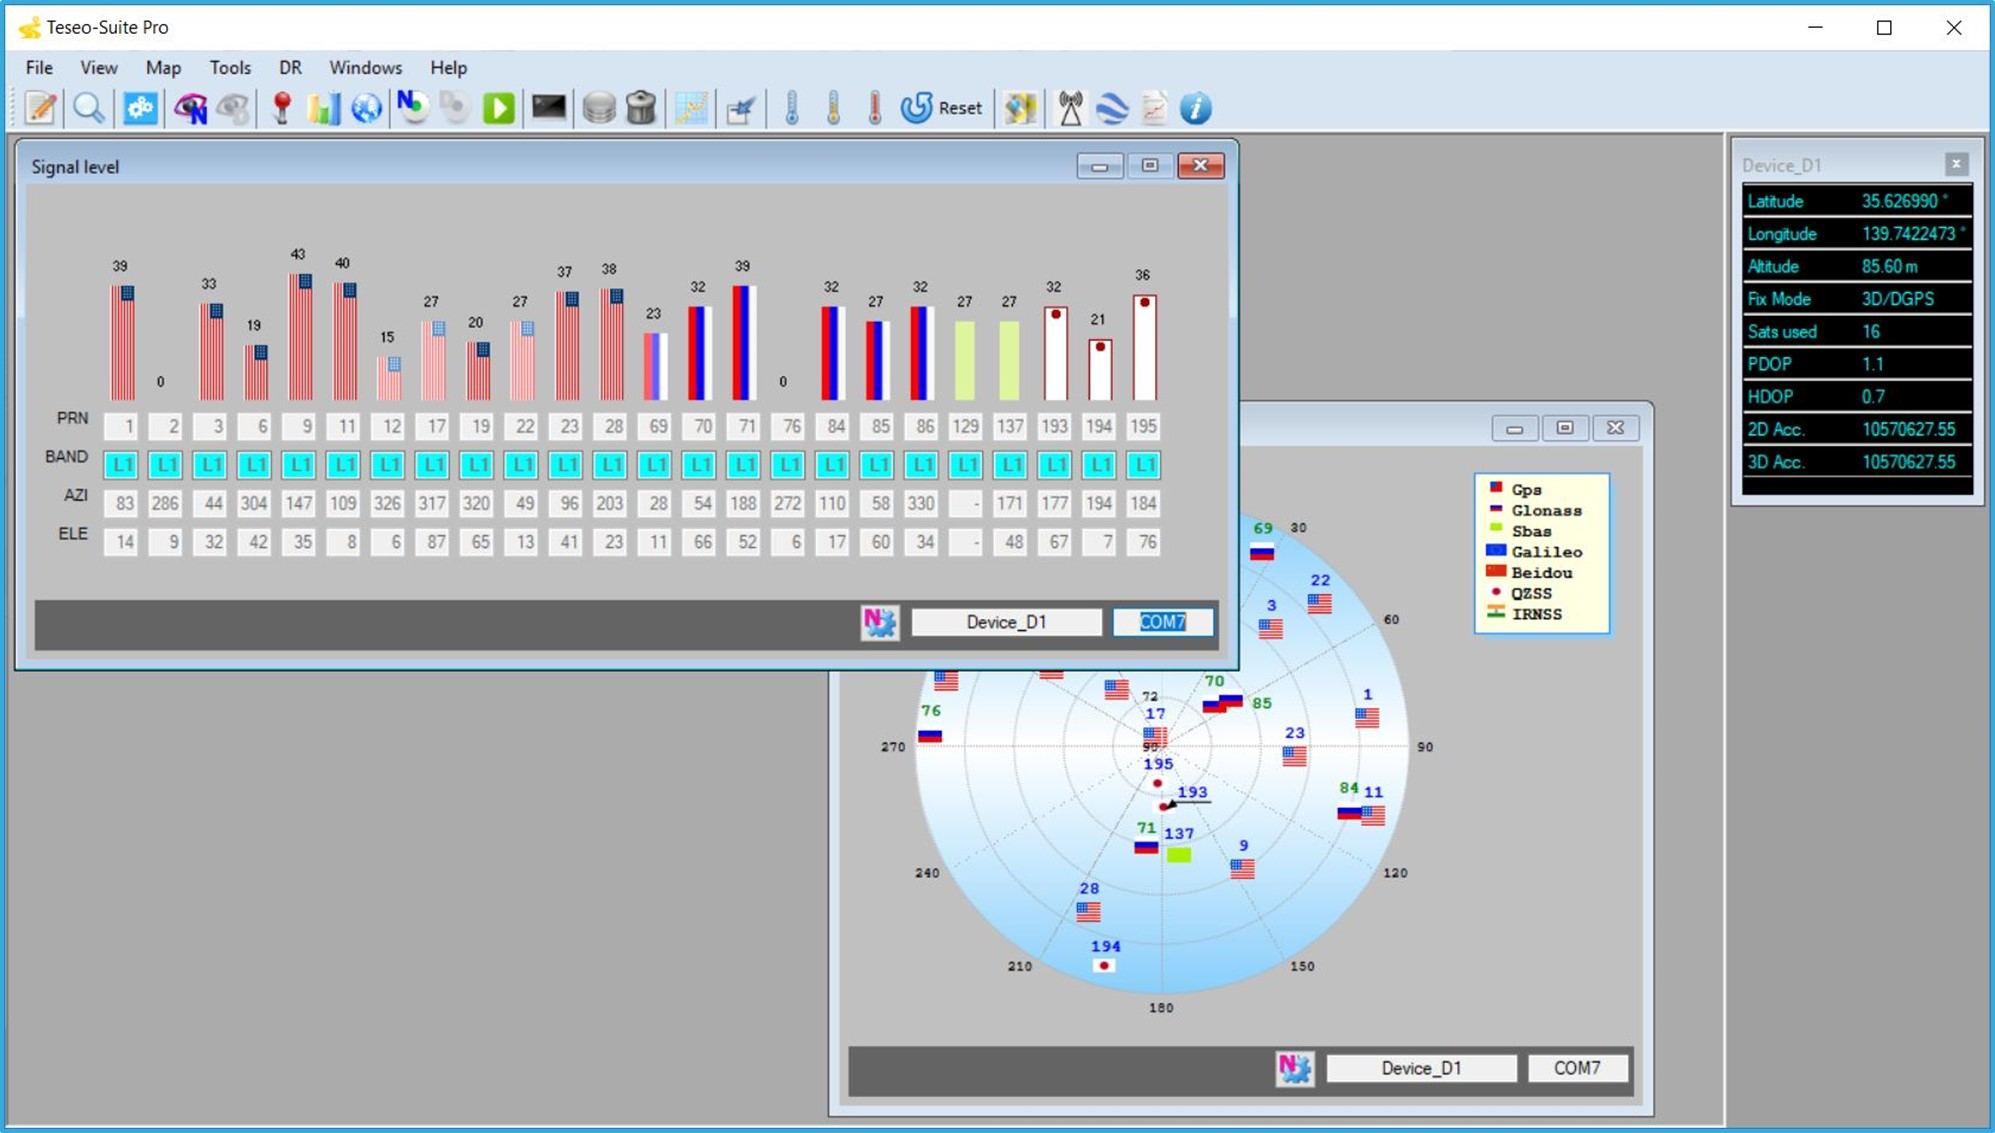
\includegraphics[width=13cm]{contents/chapter-2/teseo-suite.jpeg}
	\caption{Tampilan dari Aplikasi Teseo-Suite}
	\label{Fig: teseo-suite-ss}
\end{figure}

Tampilan dari aplikasi Teseo-Suite ditunjukkan pada Gambar \ref{Fig: teseo-suite-ss}. Pada aplikasi Teseo-Suite, pengguna dapat memvisualisasikan data satelit yang diterima oleh modul GNSS Teseo. Fitur visualisasi ini mencakup \textit{bar chart} dan \textit{sky plot} yang menunjukkan letak satelit di langit. Dengan fitur ini, pengguna dapat dengan mudah melihat satelit yang diterima oleh perangkat GNSS Teseo dan memperoleh informasi tentang nilai PRN, \textit{azimuth}, \textit{elevation}, dan pita frekuensi dari setiap satelit. Selain itu, pengguna juga dapat melihat titik koordinat pada OpenStreetMap. Fitur visualisasi ini sangat membantu pengguna dalam memahami data satelit.

\subsection{Antena \textit{Patch}}
Antena \textit{patch} adalah salah satu jenis antena yang digunakan dalam aplikasi sistem komunikasi nirkabel seperti GNSS, Wi-Fi, Bluetooth, dan sebagainya. Antena jenis ini terdiri dari sebuah \textit{patch} logam yang diletakan di atas permukaan bahan isolator. \textit{Patch} logam tersebut kemudian dihubungkan dengan kabel koaksial atau disolder langsung pada \textit{Printed Circuit Board} (PCB). Struktur dari antena \textit{patch} ditunjukan oleh Gambar \ref{Fig: patc-antenna}.

\begin{figure}[ht]
	\centering
	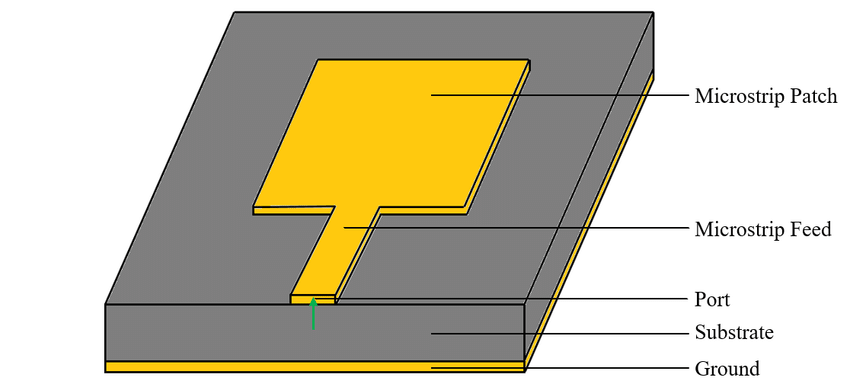
\includegraphics[width=12cm]{contents/chapter-2/patch-antena.jpg}
	\caption{Struktur dari Antena \textit{Patch} \cite{Chowdhury2019}}
	\label{Fig: patc-antenna}
\end{figure}

Keunggulan dari antena \textit{patch} adalah bentuknya ringkas dan ringan sehingga memungkinkan untuk digunakan pada aplikasi dengan dimensi kecil. Karena bentuknya kecil maka antena jenis ini hanya membutuhkan biaya yang rendah dalam manufakturnya. Selain itu, antena \textit{patch} juga memiliki \textit{gain} dan efisiensi yang tinggi \cite{Ding2020}.

Antena \textit{patch} adalah salah satu antena yang paling populer untuk aplikasi GNSS seperti pelacak, peta digital, dan navigasi kendaraan bermotor. Penggunaan antena \textit{patch} bertujuan untuk mendapatkan informasi isyarat satelit GNSS untuk kemudian diolah pada modul GNSS dengan akurasi yang tinggi.

\subsection{\textit{Universal Asynchronous Receiver Transmitter} (UART)}
\textit{Universital Asynchronous Receiver Transmitter} adalah suatu \textit{integrated circuit} (IC) yang memberikan fungsi komunikasi serial asinkron \cite{ti2010}. IC tesebut dirancang khusus untuk mengubah data paralel menjadi data serial dan menerima data serial yang dikonversi kembali menjadi data paralel. Pada komunikasi UART dibutuhkan isyarat \textit{clock} untuk sinkronisasi dan juga merupakan \textit{baud rate} dari komunikasi data yang dibangkitkan oleh masing-masing perangkat. \textit{Baud rate} tersebut dapat dipilih dalam suatu rentang tertentu. \textit{Baud rate} yang umum dipakai adalah 110, 135, 150, 300, 600, 1200, 2400, 9600, dan 115200 (bit per detik). Nilai \textit{baud rate} pada kedua perangkat harus disamakan untuk melakukan komunikasi dengan protokol ini.

 Pengiriman data pada komunikasi UART diawali dengan \textit{start bit} dan kemudian diakhiri oleh \textit{stop bit}. Data pada serial dikirimkan satu persatu melalui jalur data untuk setiap satuan waktu. Paket data diawali oleh \textit{start bit} diikuti dengan \textit{Least Significant Bit} (LSB), kemudian diikuti dengan data yang dibentuk menjadi 9-bit, dan diakhiri dengan \textit{Most Significant Bit} (MSB). Jika pengiriman data berhasil maka untuk memulai komunikasi baru dapat dilakukan dengan mengatur jalur komunikasi ke logika tinggi. Format data yang dikirimkan pada komunikasi UART ditunjukan oleh Gambar \ref{Fig: uart-format}.

\begin{figure}[H]
	\centering
	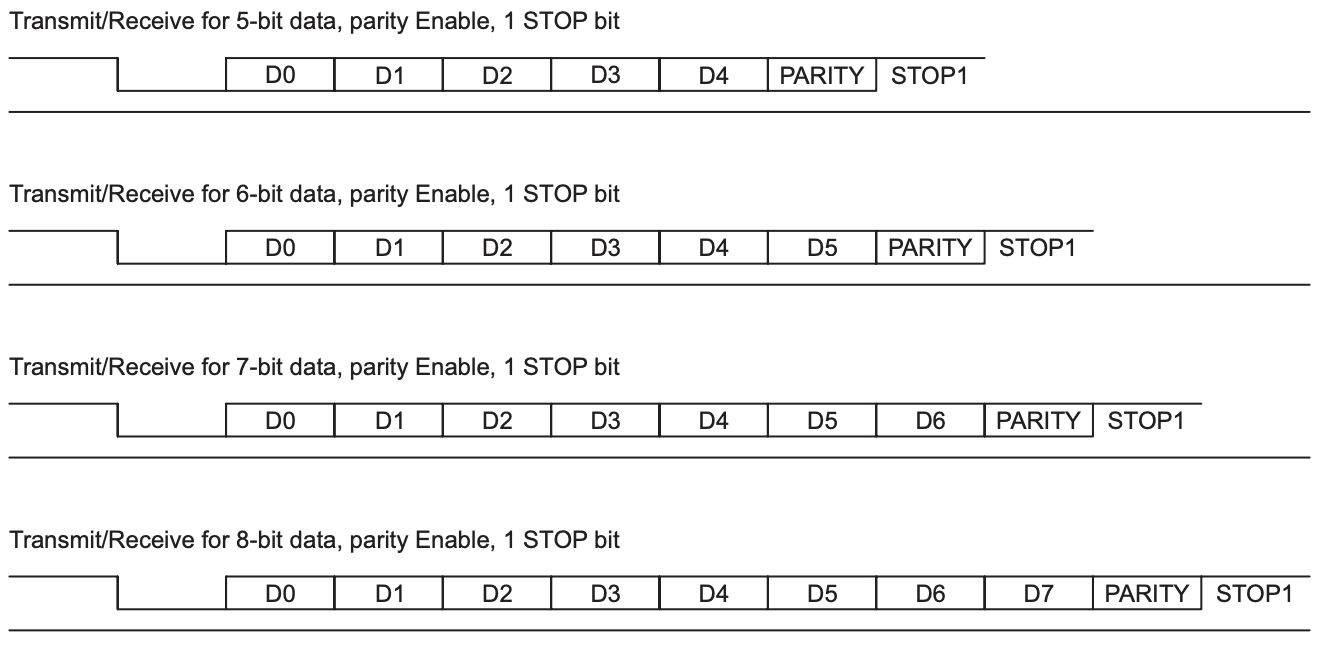
\includegraphics[width=12cm]{contents/chapter-2/uart-format.png}
	\caption{Format Data pada Komunikasi UART \cite{ti2010}}
	\label{Fig: uart-format}
\end{figure}

Pada komunikasi UART, dua perangkat dapat saling terhubung oleh dua pin TX (pengirim) dan RX (penerima). Pin TX disambungkan ke RX dan sebaliknya. Dua buah UART dapat berkomunikasi secara langsung dengan isyarat TTL dengan perangkat yang memenuhi standar ELD seperti RS-232, RS-485, dan RS-422.

\subsection{Pengolahan dan Analisis Data}

\subsubsection{Python}
Python merupakan salah satu bahasa pemrograman tingkat yang paling populer. Kepopuleran dari bahasa pemrograman Python diakibatkan bahasa pemrograman Python memiliki sintaks yang mudah dipahami. Bahasa ini dikembangkan oleh Guido van Rossum pada tahun 1991. Python dapat digunakan untuk berbagai hal seperti pengembangan web, kecerdasan buatan, dan analisis data. Selain itu Python memiliki banyak pustaka dan kerangka kerja seperti NumPy dan Matplotlib yang dapat digunakan untuk mengakselerasi pengembangan. Selain itu, bahasa ini mendukung berbagai paradigma pemrograman berorientasi objek, prosedural, maupun fungsional.

Kelebihan lain dari Python adalah kemudahan melakukan \textit{debugging} kode karena adanya kemampuan untuk mengeksekusi kode baris per baris dengan menggunakan \textit{interpreter} Python. Selain itu, Python memiliki komunitas pengguna yang besar dan aktif, sehingga memudahkan pengguna Python dalam mencari bantuan dan solusi dari masalah-masalah yang dihadapi. Oleh karena itu, Python dapat menjadi bahasa yang sangat populer di kalangan pengembang dan peneliti di berbagai bidang, terutama dalam bidang analisis dan visualisasi data.

\subsubsection{Pandas}
Pustaka Pandas merupakan alat bantu yang sangat berguna dalam mengolah dan menganalisis data. Pustaka ini dilengkapi dengan fitur-fitur struktur data yang fleksibel dan efisien seperti data frame dan series, yang memungkinkan pengguna untuk melakukan operasi pada data dengan mudah dan cepat. Selain itu, pustaka Pandas juga mendukung berbagai format file populer seperti CSV, Excel, dan basis data SQL, sehingga memudahkan pengguna untuk memproses data dari berbagai sumber.

Secara khusus, struktur data Pandas yang disebut sebagai data frame merupakan kumpulan kolom data yang diberi nama dan jenis tertentu. Dengan adanya fitur data frame, pengguna dapat dengan mudah membaca file dan mengubahnya menjadi sebuah tabel. Data frame juga memungkinkan pengguna untuk melakukan operasi seperti \texttt{join}, \texttt{distinct}, \texttt{group by}, dan fitur lainnya yang biasa ditemukan pada SQL. Pustaka Pandas juga mendukung berbagai format file seperti .txt, .csv, .tsv, dan lainnya, sehingga memudahkan pengguna dalam mengakses berbagai jenis data.

\subsubsection{NumPy}
Selain pustaka Pandas, NumPy (\textit{Numerical Python}) juga memainkan peran penting dalam pengolahan data. NumPy terutama digunakan untuk operasi numerik pada data dan menyediakan berbagai struktur data seperti larik dan matriks multidimensi, serta berbagai fungsi matematika yang sangat penting dalam pengolahan data. NumPy dikembangkan menggunakan bahasa pemrograman C, yang memungkinkan komputasi yang cepat dan optimal pada pengolahan data yang kompleks.

NumPy sangat berguna dalam bidang ilmu data dan analisis data. Dalam analisis data, NumPy memungkinkan pengolahan data yang efisien dan cepat, seperti pengolahan gambar, pemrosesan isyarat, dan analisis numerik lainnya. Struktur data seperti larik dan matriks multidimensi yang disediakan oleh NumPy sangat membantu dalam pengolahan data. Kinerja yang cepat dan efisien dari NumPy memungkinkan analisis data yang lebih cepat dan akurat.

\subsubsection{PyNMEA2}
Pustaka PyNMEA2 merupakan pustaka Python yang berguna dalam melakukan pengolahan data yang dihasilkan oleh modul GNSS seperti Teseo-LIV3FL. Modul GNSS ini sangat umum digunakan dalam kegiatan navigasi dan survei di berbagai sektor seperti industri, pertanian, kelautan, dan lain-lain. Dalam kegiatan tersebut, data yang dihasilkan oleh modul GNSS harus diproses lebih lanjut agar dapat memberikan informasi yang akurat dan bermanfaat.

PyNMEA2 memiliki kemampuan untuk melakukan penguraian terhadap berbagai jenis kalimat NMEA yang dihasilkan oleh modul GNSS, seperti GPGGA, GNGSA, GPRMC, dan lain-lain. Dalam proses pengolahan data, PyNMEA2 dapat mempermudah proses ekstrasi data dari hasil pengamatan.Dengan menggunakan pustaka ini, data dari setiap kalimat NMEA dapat diekstraksi dan diproses lebih lanjut.

\subsubsection{Matplotlib}
Untuk melakukan visualisasi data yang telah diolah akan digunakan pustaka Matplotlib. Pustaka ini adalah pustaka paling populer dalam bidang visualisasi data. Secara bawaan, Matplotlib menyediakan berbagai jenis visualisasi data seperti \textit{line plot}, \textit{scatter plot}, \textit{histogram}, \textit{bar plot}, dan lain-lain secara bawaan. Seluruh jenis visualisasi tersebut dapat dikustomisasi sesuai dengan kebutuhan pengguna, mulai dari mengubah warna, ukuran, jenis garis, dan sebagainya. Bahkan pengguna dapat menambahkan elemen visual seperti judul, label sumbu, dan legenda dengan mudah.

\subsubsection{Seaborn}
Terakhir, Seaborn adalah pustaka Python yang digunakan untuk membuat plot statistik yang menarik dan informatif. Pustaka ini dibangun di atas Matplotlib, sehingga menggabungkan kekuatan dari kedua pustaka tersebut dapat menghasilkan plot yang lebih baik secara visual dan informasi. Dalam implementasinya, Seaborn dapat digabungkan dengan Matplotlib untuk menghasilkan plot yang lebih baik secara visual dan informatif. Penggunaan Seaborn dapat digunakan untuk memperbaiki plot Matplotlib standar dengan memberikan warna bawaan yang lebih baik dan meningkatkan aspek visual dari grafik.

\iffalse
\subsection{LoRa}
Teknologi \textit{Long Range} (LoRa) adalah protokol komunikasi pada lapiran fisik yang memungkinkan untuk mentransmisikan isyarat pada jarak jauh dengan konsumsi daya seminimal mungkin. LoRa diperkenalkan oleh Semtech pada tahun 2012 \cite{Oliveira2017}. Pada teknologi LoRa digunakan frekuensi \textit{sub-GHZ} 433 MHz di Asia. Indonesia menggunakan standar frekuensi 920-923MHz (AS923-2) \cite{LoRa2020}.

Tiga alasan yang membuat teknologi LoRa banyak digunakan dalam industri:

\begin{enumerate}
	\item Menurut penelitian \cite{Petajajarvi2016} dan \cite{Haxhibeqiri2017}, pada kondisi tanpa halangan dimungkinkan untuk mentransmisikan jarak pada radius 2-5 km. Pada kondisi dengan penghalang seperti gedung dan pepohonan dimungkinkan untuk transmisi data hingga 2 km \cite{Rida2019}.
	\item Perangkat LoRa dibuat sesederhana mungkin. Kompleksivitas yang rendah memungkinkan untuk menekan biaya manufaktur.
	\item Teknologi LoRa menggunakan daya sebesar 120-150mW sehingga dapat memperpanjang umur dari perangkat hingga 2-5 tahun.
\end{enumerate}

\subsubsection{LoRaWAN}
LoRa dan LoRaWAN adalah dua hal yang berbeda. Lora adalah teknik modulasi yang digunakan untuk komunikasi antar \textit{end node} atau \textit{end node} dengan \textit{gateway}, sedangkan LoRaWAN adalah arsitektur jaringan yang memungkinkan perangkat LoRaWAN untuk mengirimkan data ke \textit{server} LoRaWAN \cite{Zhou2019}. Arsitektur LoRaWAN ditunjukan oleh Gambar \ref{Fig: lorawan-architecure}.
\begin{figure}[ht]
	\centering
	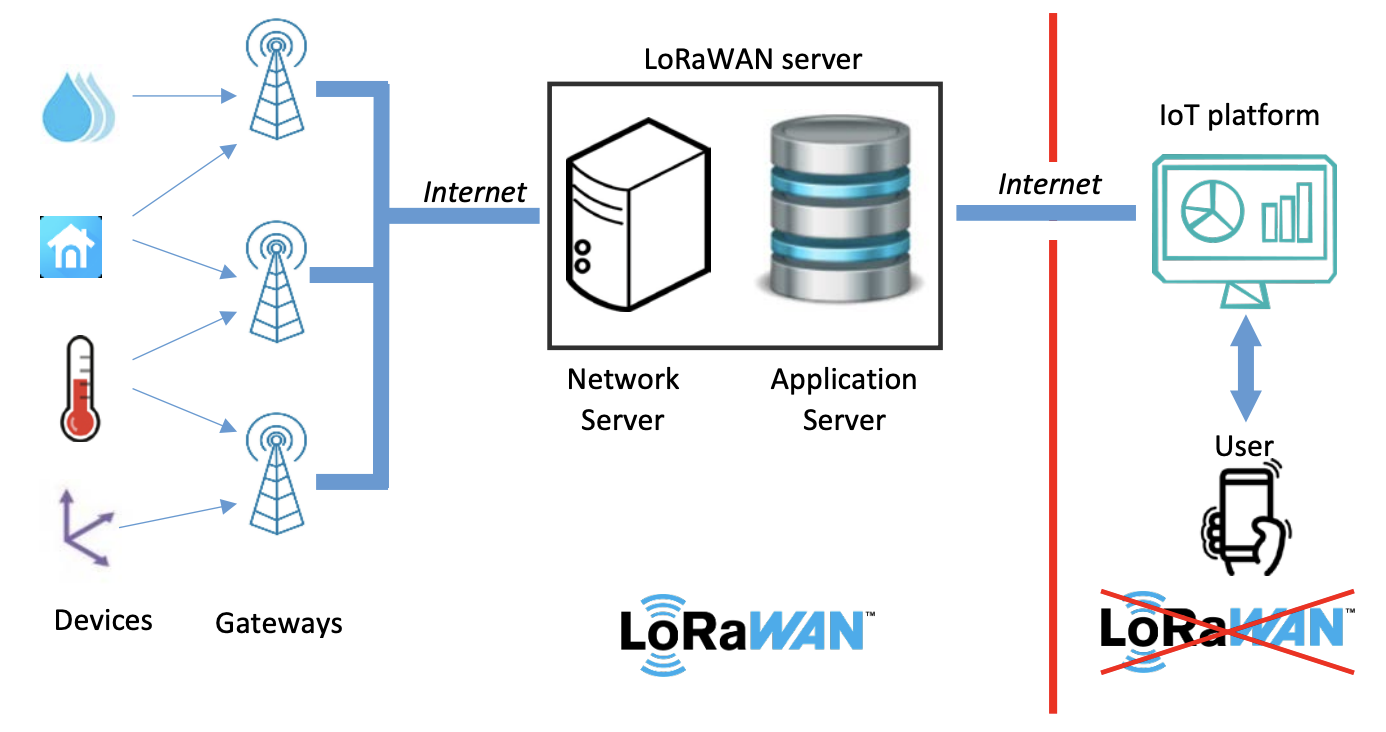
\includegraphics[width=13cm]{contents/chapter-2/lorawan-architecture.png}
	\caption{Arsitektur Jaringan LoRaWAN \cite{Montagny2022}}
	\label{Fig: lorawan-architecure}
\end{figure}

Lapisan fisik LoRa adalah teknologi yang dimiliki oleh Semtech, sedangkan LoRaWAN adalah standar umum yang dikelola oleh Lora Alliance \cite{Augustin2016}. 

\subsubsection{Metode Aktivasi}
Terdapat dua metode aktivasi pada perangkat \textit{end node}, yaitu \textit{Over the Air Activation} (OTAA) dan \textit{Activation by Personalization} (ABP).

\textbf{\textit{Over the Air Activation} (OTAA)} adalah metode aktivasi yang hanya membutuhkan AppEUI, DevEUI, dan AppKey. Pada metode aktivasi OTAA, alamat perangkat DevAddr diberikan ke perangkat \textit{end device} dengan \textit{root keys} untuk membuat \textit{session keys}. Oleh karena itu, DevAddr dan \textit{session keys} berubah setiap \textit{session} baru dibuat \cite{LoRa2017}. Pada penelitian ini digunakan metode aktivasi OTAA karena metode aktivasi OTAA lebih aman jika dibandingkan dengan ABP.

EUI atau \textit{Extended Unique Identifier} berperan sebagai identifikasi dengan panjang 64-bit. DevEUI bersifat unik untuk setiap perangkat. AppKey atau \textit{root key} memiliki panjang 128-bit digunakan untuk menghasilkan \textit{Message Integrity Code} (MIC) sebagai verifikasi integritas pesan. Nilai AppKey harus disimpan pada \textit{end node} dan \textit{network server}.

\textbf{\textit{Activation by Personalization} (ABP)} adalah metode aktivasi yang lebih sederhana dibandingkan dengan OTAA. Pada metode aktivasi ABP, nilai DevAddr dan \textit{session keys} bersifat statik.
\fi